In diesem abschließenden Kapitel möchten wir die Ergebnisse der in
\Cref{chap:implementation} beschriebenen Realisierung von
\Cref{alg:primalDualIteration} mit Abbruchkriterium
\eqref{eq:terminationCriterion} im Solve-Schritt der AFEM-Schleife aus
\Cref{fig:afemLoop} untersuchen, deren initiales Level dabei mit 0 nummeriert
wird.
Bezüglich einer Triangulierung $\Tcal$ schreiben wir hier $\ucrt$ und
$\bar\Lambda_{0,\Tcal}$ für $\ucr$ und $\bar\Lambda_0$ aus
\Cref{thm:convergenceIteration} sowie $(\ujt, \Lambda_{j,\Tcal})_{j\in\Nbb}$
für die Iterate $\left(u_j, \Lambda_j\right)_{j\in\Nbb}$  von
\Cref{alg:primalDualIteration}.
Zunächst möchten wir die Belegung für alle Parameter aus den Tabellen
\ref{tab:paramsMisc}--\ref{tab:paramsExperiment}, die für ein Experiment
relevant sind, festlegen.
Die Wahlen $\tau = 1$ für \Cref{alg:primalDualIteration} und $\epsstop
= 10^{-4}$ für das Abbruchkriterium \eqref{eq:terminationCriterion} begründen
wir in \Cref{sec:choiceOfParameters} experimentell. 
Außerdem nutzen wir $\gamma = 1$ für den Parameter $\gamma$ des
Verfeinerungsindikators aus \Cref{def:refinementIndicator}, wobei wir den
Einfluss dieses Parameters auf das Programm in
\Cref{sec:experimentsWithExactSolution} untersuchen. 
Eine Übersicht über alle somit festgelegten Standardwerte ist in
\Cref{tab:parameterStandardValues} zu finden. 
Wir werden in einem Experiment die Wahl eines Parameters nur
erwähnen, wenn diese vom Standardwert abweicht.
In \Cref{tab:usedBenchmarks} wird für alle verwendeten Benchmark-Datein
aufgelistet, für welche Abbildungen die Ergebnisse des entsprechenden
Programmaufrufs genutzt wurden.

\begin{table}[p]
  \centering
  \begin{tabular}{c|p{9.5cm}}
    \hline 
    Parametername & Standardwert\\
    \hline 
    \texttt{degree4Integrate}&
    $10$\\
    \texttt{geometry} &
    \texttt{'BigSquare'} für Experimente mit bekannter exakter Lösung \newline
    \texttt{'Square'} für Experimente mit Graufarbenbild als Eingangssignal\\
    \texttt{initialRefinementLevel} &
    $0$\\
    \texttt{parTheta}, $\theta$ &
    $0.5$\\
    \texttt{minNrDof} &
    $10^8$\\
    \texttt{useProlongation} &
    \texttt{true}\\
    \texttt{parGamma}, $\gamma$ &
    $1$\\
    \texttt{d}, $d$ &
    $2$\\
    \texttt{u0Mode} &
    \texttt{zeros}\\
    \texttt{epsStop}, $\epsstop$ &
    $10^{-4}$\\
    \texttt{parTau}, $\tau$ &
    $1$\\
    \texttt{maxIter} &
    $10^{12}$\\
    \texttt{parAlpha}, $\alpha$ &
    $\alpha$ für Experimente mit Eingangssignal $f_\alpha$\newline
    $10^4$ für Experimente mit Eingangssignal \texttt{cameraman} \\
    \texttt{parBeta}, $\beta$ &
    $1$ für Experimente mit Eingangssignal $f_\alpha$\\
    \hline
  \end{tabular}
  \caption{Wahl der relevanten Parameter für die Experimente}
  \label{tab:parameterStandardValues}
\end{table} 
\begin{table}[p]
  \centering
  \begin{tabular}{c|p{8.7cm}}
    \hline
    \texttt{benchmark} & Abbildungen\\  
    \hline 
    \texttt{denoiseAlpha100} &
    \ref{fig:snr15alpha100}\\
    \texttt{denoiseAlpha1000} &
    \ref{fig:snr15alpha1000}\\
    \texttt{denoiseAlpha2500} &
    \ref{fig:snr15alpha2500}\\
    \texttt{denoiseAlpha5000} &
    \ref{fig:snr15alpha5000}\\
    \texttt{denoiseAlpha10000} &
    \ref{fig:snr15alpha10000}\\
    \texttt{denoiseAlpha50000} &
    \ref{fig:snr15alpha50000}\\
    \texttt{paramsTau\_f01\_0Dot1} &
    \ref{fig:parTauMiscF}, \ref{fig:parTauConvergence},
    \ref{fig:iterationEnergyOscillations}\\
    \texttt{paramsTau\_f01\_0Dot5} &
    \ref{fig:parTauMiscF}, \ref{fig:parTauConvergence}\\
    \texttt{standard\_f01} &
    \ref{fig:parTauMiscF}, \ref{fig:parTauConvergence}, 
    \ref{fig:iterationEnergyLevel}, \ref{fig:iterationTermination},
    \ref{fig:f01Convergence}, \ref{fig:f01SolAdaptive},
    \ref{fig:f01SupplementaryInfo}, \ref{fig:parGammaConvergence},
    \ref{fig:gamma1Triang}, \ref{fig:inSiNrIterComparison}\\
    \texttt{paramsTau\_cameraman\_0Dot1} &
    \ref{fig:parTauMiscCam}\\
    \texttt{paramsTau\_cameraman\_0Dot5} &
    \ref{fig:parTauMiscCam} \\
    \texttt{standard\_cameraman} &
    \ref{fig:parTauMiscCam}, \ref{fig:camConvergence}, \ref{fig:camTriang}\\
    \texttt{noTerminationTau\_maxIter1e5} &
    \ref{fig:parTauNoConvergence}\\
    \texttt{paramsEpsStop\_1em2} &
    \ref{fig:parEpsStopConvergence}\\
    \texttt{paramsEpsStop\_1em3} &
    \ref{fig:parEpsStopConvergence}\\
    \texttt{paramsEpsStop\_1em4} &
    \ref{fig:parEpsStopConvergence}\\
    \texttt{paramsEpsStop\_1em5} &
    \ref{fig:parEpsStopConvergence}\\
    \texttt{standardUniform\_f01} &
    \ref{fig:f01Convergence}, \ref{fig:f01SupplementaryInfo}\\
    \texttt{standard\_f01Alpha1e4} &
    \ref{fig:f01LargeAlphaConvergence}, \ref{fig:inSiNrIterComparison}\\
    \texttt{standardUniform\_f01Alpha1e4} &
    \ref{fig:f01LargeAlphaConvergence}\\
    \texttt{parGamma\_0} &
    \ref{fig:parGammaConvergence}, \ref{fig:gamma0Triang}\\
    \texttt{parGamma\_0Dot5} &
    \ref{fig:parGammaConvergence}, \ref{fig:gammaDot5Triang}\\
    \texttt{standard\_f04} &
    \ref{fig:f04Convergence}, \ref{fig:inSiNrIterComparison}\\
    \texttt{standardUniform\_f04} &
    \ref{fig:f04Convergence}\\
    \texttt{standardUniform\_cameraman} &
    \ref{fig:camConvergence}\\
    \texttt{circleContinuousAdaptive} &
    \ref{fig:circConvAdaptive}, \ref{fig:circContConvergence},
    \ref{fig:circContLvl17Triang}, %\ref{fig:circContFinalTriang},
    \ref{fig:circContSol}, \ref{fig:circContSolAxis}\\
    \texttt{circleDiscontinuousAdaptive} &
    \ref{fig:circConvAdaptive}\\
    \texttt{circleContinuousUniform} &
    \ref{fig:circConvUniform}, \ref{fig:circContConvergence},
    \ref{fig:circDiscLvl17Triang}, %\ref{fig:circDiscFinalTriang},
    \ref{fig:circDiscSol}, \ref{fig:circDiscSolAxis}\\
    \texttt{circleDiscontinuousUniform} &
    \ref{fig:circConvUniform}\\
    \hline
  \end{tabular}
  \caption{Eingabeparameter \texttt{benchmark} für \texttt{startAlgorithmCR},
    um die Rechnung zu einem Experiment zu starten, und die Abbildungen, die
    auf den Ergebnissen dieses Experiments basieren} 
  \label{tab:usedBenchmarks}
\end{table} 

Als Startwert für die primale-duale Iteration des ersten Levels der
AFEM-Routine wählen wir $u_0\equiv 0$. 
Für die Iteration der darauffolgenden Level wählen wir die zum Ende von
\Cref{sec:programFlow} beschriebene Prolongation des Ergebnisses des
jeweils vorherigen Levels.
In allen Experimenten hatte dadurch die Wahl der Startwerts für die Iteration
des ersten Levels keinen nennenswerten Einfluss auf die Dauer des Experiments
oder die Güte der Ergebnisse. 
Für jeden Aufruf der primalen-dualen Iteration auf einer Triangulierung $\Tcal$
wählen wir dann $\Lambda_{0,\Tcal}$ wie in
\Cref{eq:choiceInitialDualVariableImplementation} angegeben.
Eingangssignale für Experimente, bei denen die exakte
Lösung bekannt ist, konstruieren wir nach \Cref{sec:constructionInputSignal}.
Die schwachen Ableitungen dieser Eingangssignale und der entsprechenden exakten
Lösungen berechnen wir ebenfalls nach \Cref{sec:constructionInputSignal}.
Dabei sei das Argument $r$ einer Funktion stets aus $[0,\infty)$.
\begin{figure}[p]
  \centering
  \begin{subfigure}[b]{.48\linewidth}
    \centering
    \caption{\texttt{BigSquare}}
    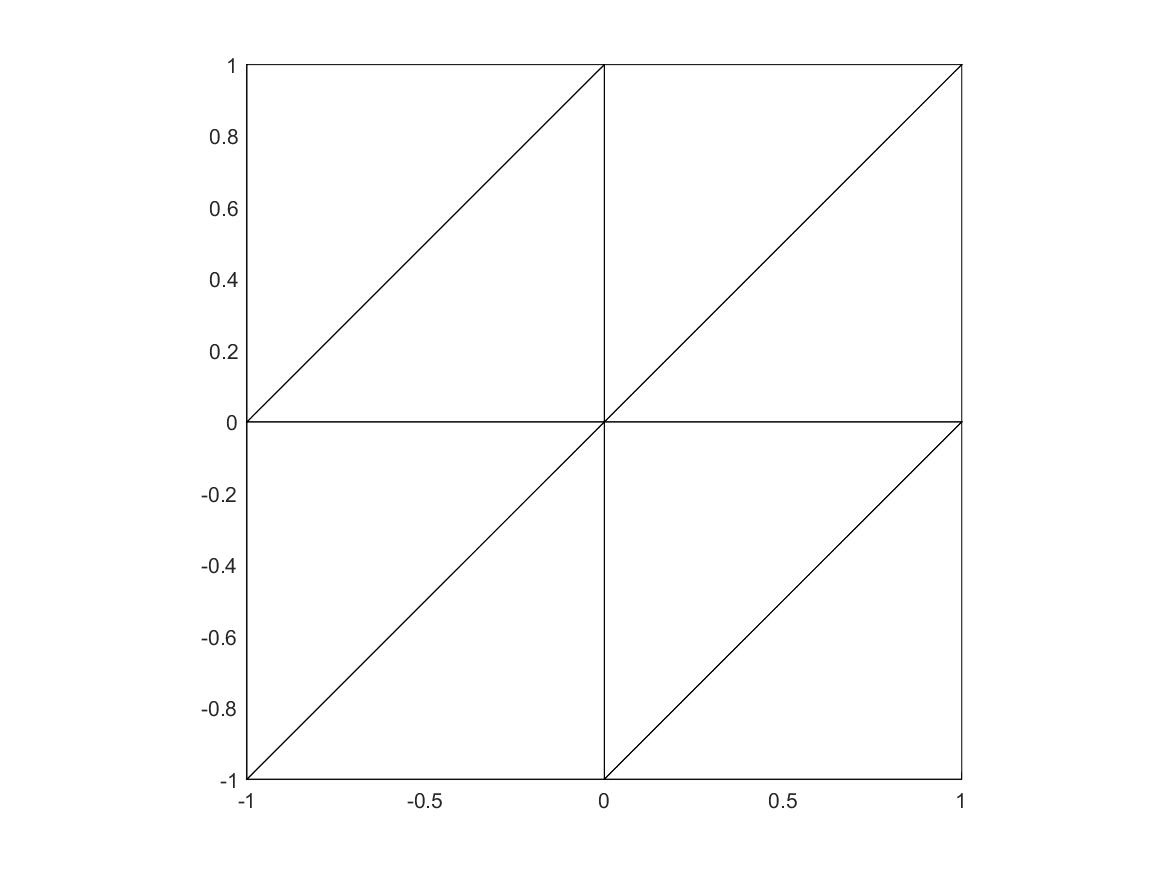
\includegraphics[trim = 90 30 90 20, clip, width=\linewidth]
      {pictures/chapExperiments/secGeneralInfo/bigSquareTriang.png}
    \label{fig:triangBigSquare}
  \end{subfigure}
  \quad
  \begin{subfigure}[b]{.48\linewidth}
    \centering
    \caption{\texttt{Square}}
    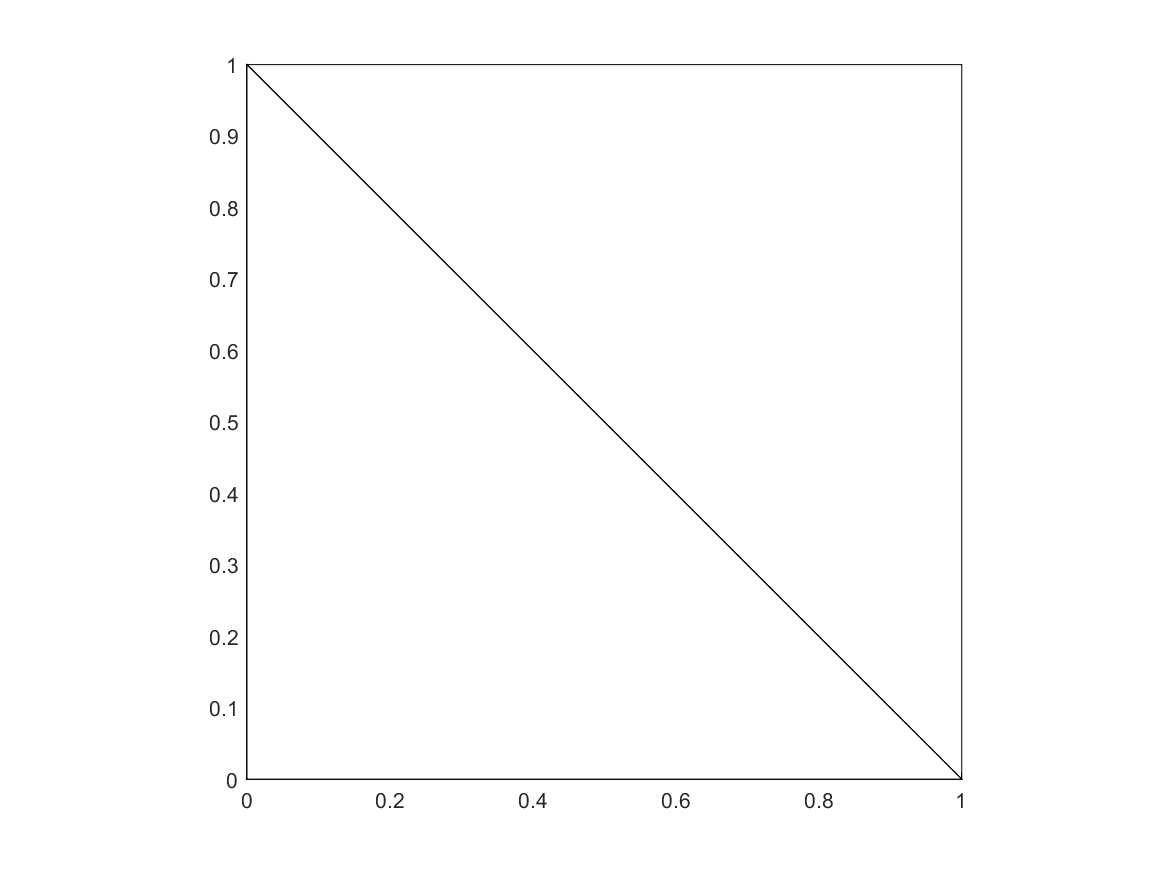
\includegraphics[trim = 90 30 90 20, clip, width=\linewidth]
      {pictures/chapExperiments/secGeneralInfo/squareTriang.png}
    \label{fig:triangSquare}
  \end{subfigure}
  \caption{Initiale Triangulierung für Experimente mit bekannter exakter Lösung
    (a) und für Experimente mit Graufarbenbild als Eingangssignal (b)}
  \label{fig:initialTriangulations}
\end{figure}
Als Geometrie für das erste Level des AFEM-Al\-go\-rith\-mus nutzen wir in
Experimenten mit bekannter exakter Lösung die Triangulierung aus
\Cref{fig:triangBigSquare} und in Experimenten mit einem Graufarbenbild als
Eingangssignal die Triangulierung aus \Cref{fig:triangSquare}.
Wir nutzen adaptive Netzverfeinerungen und dafür den Bulk-Parameter
$\theta=0.5$ für den Mark-Schritt des AFEM-Algorithmus und dem Parameter
$\gamma=1$ für den Verfeinerungsindikator aus \Cref{def:refinementIndicator}.
Die maximale Iterationszahl wurde mit $10^{12}$ so gewählt, dass diese nie
Grund für das Beenden der primalen-dualen Iteration war.
Dementsprechend ist das Abbruchkriterium aus \eqref{eq:terminationCriterion}
für den Abbruch der Iteration verantwortlich.
Die minimale Anzahl der Freiheitsgrade, welche eine Triangulierung während der
AFEM-Routine zum Abbrechen erreichen soll, ist mit $10^8$ so gewählt, dass die
verfügbaren Ressourcen des verwendeten Rechners in der Regel ausgenutzt
werden und die Rechnungen manuell beendet werden müssen.
Dies geschah in allen Experimenten bei ungefähr $10^6$ Freiheitsgraden.
Beispielrechnungen mit verschiedenen Eingangssignalen ergaben, dass deutlich
höhere Integrationsgrade als $10$ zu keinen veränderten Konvergenzraten
führen. 
Diese Wahl des Integrationsgrads erscheint daher als ausreichend.
Da außerdem die \texttt{integrate} Methode des AFEM-Softwarepakets \cite{Car09}
nicht während der primalen-dualen Iteration aufgerufen werden muss, hat eine
möglicherweise zu hohe Wahl des Integrationsgrads keinen signifikanten Einfluss
auf die Programmlaufzeit.
Nur die Methode \texttt{errorCRL2} des AFEM-Softwarepakets, die zur Berechnung
des exakten $L^2$-Fehlers verwendet wird, nutzt den Integrationsgrad 12, da
diese unverändert übernommen wurde.

Nun möchten wir ein Eingangssignal definieren, welches in mehreren der
folgenden Abschnitte verwendet wird.
Sei $\beta\geq 1/2$, wobei wir stets $\beta=1$ wählen. 
Wir betrachten die Funktion
\begin{align*}
  u(r)&\coloneqq
  \begin{cases}
    1, 
    & \text{falls } r\in \left[0,\frac{1}{6}\right]\!,\\
    1+(6r-1)^\beta, 
    & \text{falls } r\in \left(\frac{1}{6}, \frac{1}{3}\right]\!,\\
    2, 
    & \text{falls } r\in \left(\frac{1}{3}, \frac{1}{2}\right]\!,\\
    2\left(\frac{5}{2}-3r\right)^\beta, 
    & \text{falls } r\in \left(\frac{1}{2}, \frac{5}{6}\right]\!,\\
    0, 
    & \text{falls } r\in \left(\frac{5}{6}, \infty\right)\!,\\
  \end{cases}
\end{align*}
und wählen
\begin{align*}
  \sgn\big(\partial_r u(r)\big) 
  &\coloneqq
  \begin{cases}
    12r-36r^2, 
    & \text{falls } r\in \left[0,\frac{1}{6}\right]\!,\\
    1, 
    & \text{falls } r\in \left(\frac{1}{6}, \frac{1}{3}\right]\!,\\
    \cos(\pi(6r-2)), 
    & \text{falls } r\in \left(\frac{1}{3}, \frac{1}{2}\right]\!,\\
    -1, 
    & \text{falls } r\in \left(\frac{1}{2}, \frac{5}{6}\right]\!,\\
    -\frac{1+\cos(\pi(6r-5))}{2}, 
    & \text{falls } r\in \left(\frac{5}{6}, \infty\right)\!.
  \end{cases}
\end{align*}
Nach \Cref{eq:constructionInputSignal} ist $u$ mit dieser Wahl von
$\sgn\big(\partial_r u\big)$ die Lösung von \Cref{prob:continuousProblem} mit
Eingangssignal
\begin{align*}
  f_\alpha(r)
  &=
  \begin{cases}
    \alpha-12(2-9r), 
    & \text{falls } r\in \left[0,\frac{1}{6}\right]\!,\\
    \alpha\left(1+(6r-1)^\beta\right)-\frac{1}{r}, 
    & \text{falls } r\in \left(\frac{1}{6}, \frac{1}{3}\right]\!,\\
    2\alpha+6\pi\sin(\pi(6r-2))-\frac{1}{r}\cos(\pi(6r-2)), 
    & \text{falls } r\in \left(\frac{1}{3}, \frac{1}{2}\right]\!,\\
    2\alpha\left(\frac{5}{2}-3r\right)^\beta+\frac{1}{r},
    & \text{falls } r\in \left(\frac{1}{2}, \frac{5}{6}\right]\!,\\
    -3\pi\sin(\pi(6r-5))+\frac{1+\cos(\pi(6r-5))}{2r}, 
    & \text{falls } r\in \left(\frac{5}{6}, \infty\right)\!.
  \end{cases}
\end{align*}
Dieses Eingangssignal für zwei Wahlen von $\alpha$ und die exakte Lösung $u$
von \Cref{prob:continuousProblem} mit Eingangssignal $f_\alpha$ können in
\Cref{fig:f01Plots} betrachtet werden.
Wir können anhand von \Cref{fig:f01Plots} ebenfalls den in
\Cref{chap:introduction} beschriebenen Zusammenhang von
\Cref{prob:continuousProblem} und dem ROF-Modell sehen, denn für $\alpha=10^4$
scheint annähernd $f_\alpha=\alpha u$ zu gelten.
\begin{figure}[p]
  \centering
  \begin{subfigure}[b]{.48\linewidth}
    \centering
    \caption{$f_1$}
    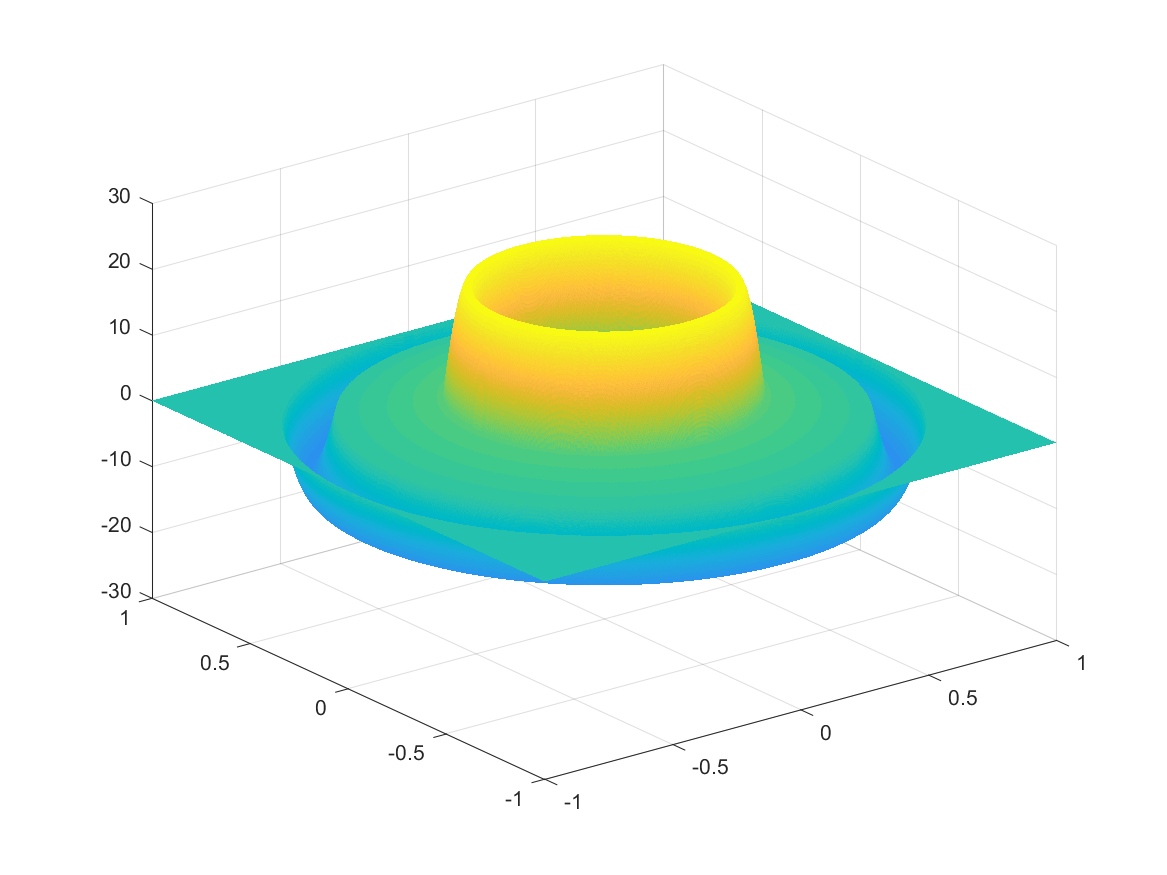
\includegraphics[trim = 40 30 30 30, clip, width=\linewidth]
      {pictures/chapExperiments/secGeneralInfo/f01Plots/inSi1.png}
    \label{fig:f01InSi}
  \end{subfigure}
  \quad
  \begin{subfigure}[b]{.48\linewidth}
    \centering
    \caption{$f_1$ entlang der x- und y-Achse}
    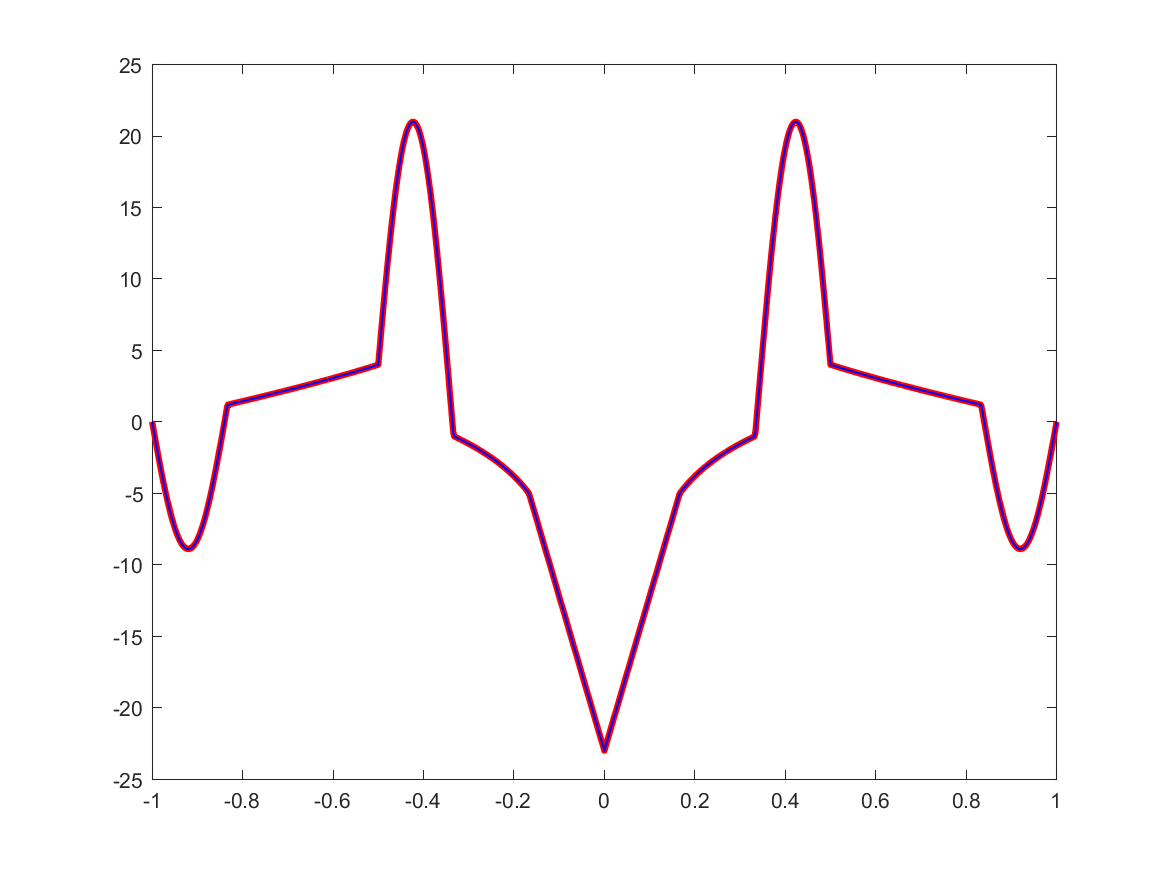
\includegraphics[trim = 50 30 50 20, clip, width=\linewidth]
      {pictures/chapExperiments/secGeneralInfo/f01Plots/inSi1Axis.png}
    \label{fig:f01InSiAxis}
  \end{subfigure}

  \begin{subfigure}[b]{.48\linewidth}
    \centering
    \caption{$f_{10^4}$}
    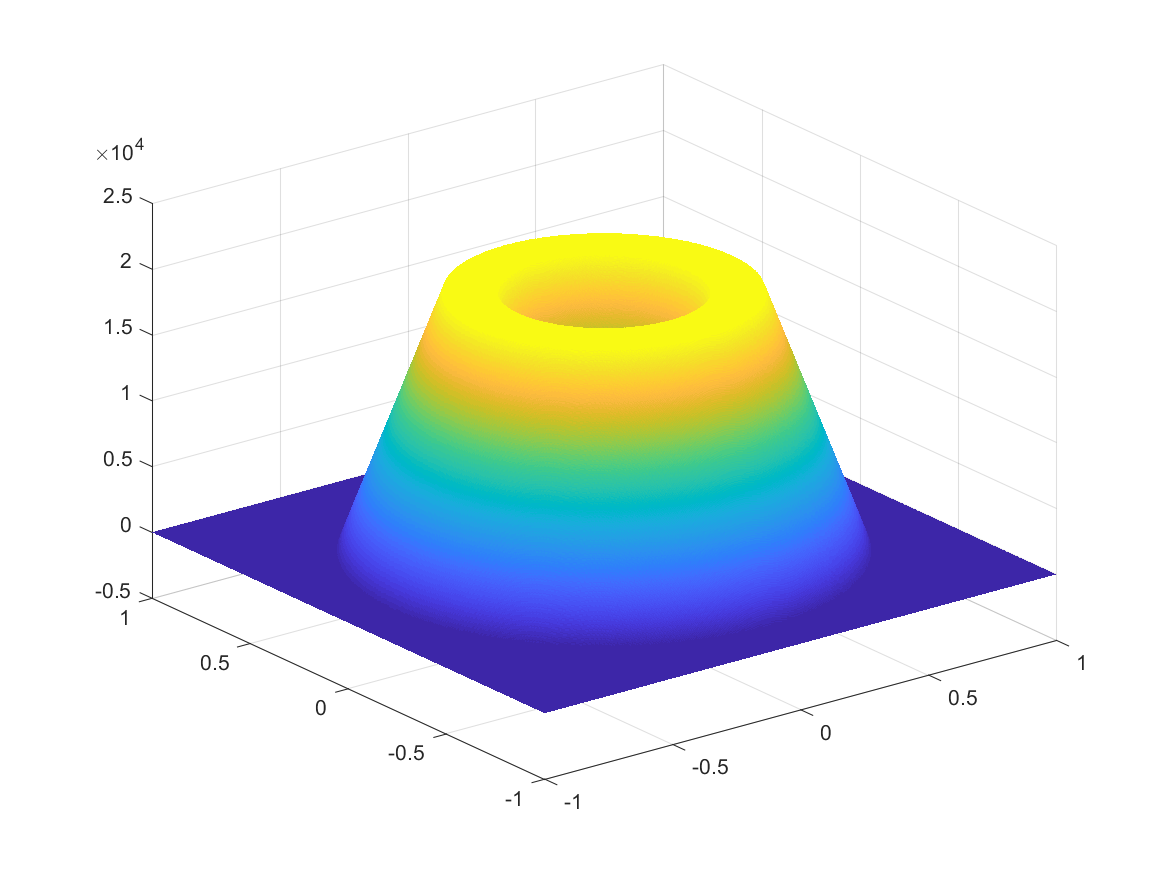
\includegraphics[trim = 40 30 30 30, clip, width=\linewidth]
      {pictures/chapExperiments/secGeneralInfo/f01Plots/inSi1e4.png}
    \label{fig:f01AlphaLargeInSi}
  \end{subfigure}
  \quad
  \begin{subfigure}[b]{.48\linewidth}
    \centering
    \caption{$f_{10^4}$ entlang der x- und y-Achse}
    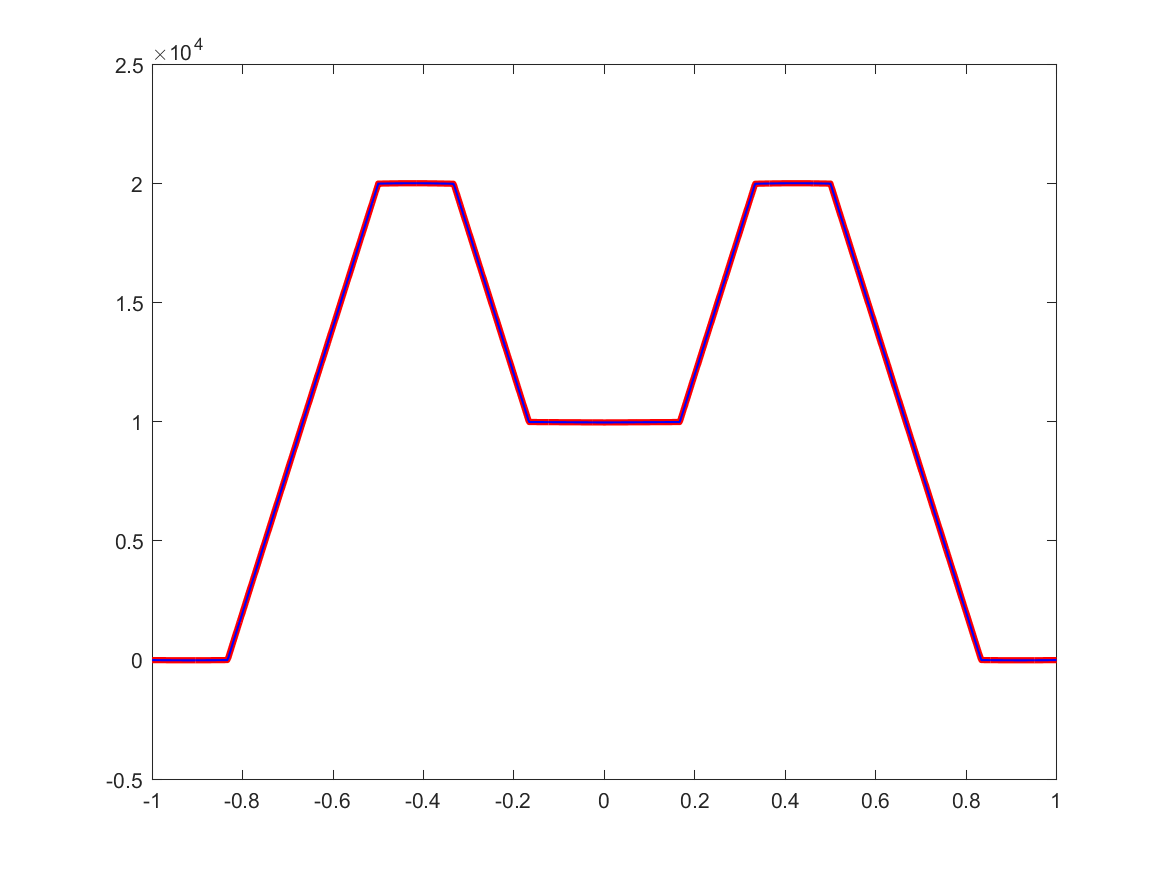
\includegraphics[trim = 50 30 50 20, clip, width=\linewidth]
      {pictures/chapExperiments/secGeneralInfo/f01Plots/inSi1e4Axis.png}
    \label{fig:f01AlphaLargeInSiAxis}
  \end{subfigure}

  \begin{subfigure}[b]{.48\linewidth}
    \centering
    \caption{$u$}
    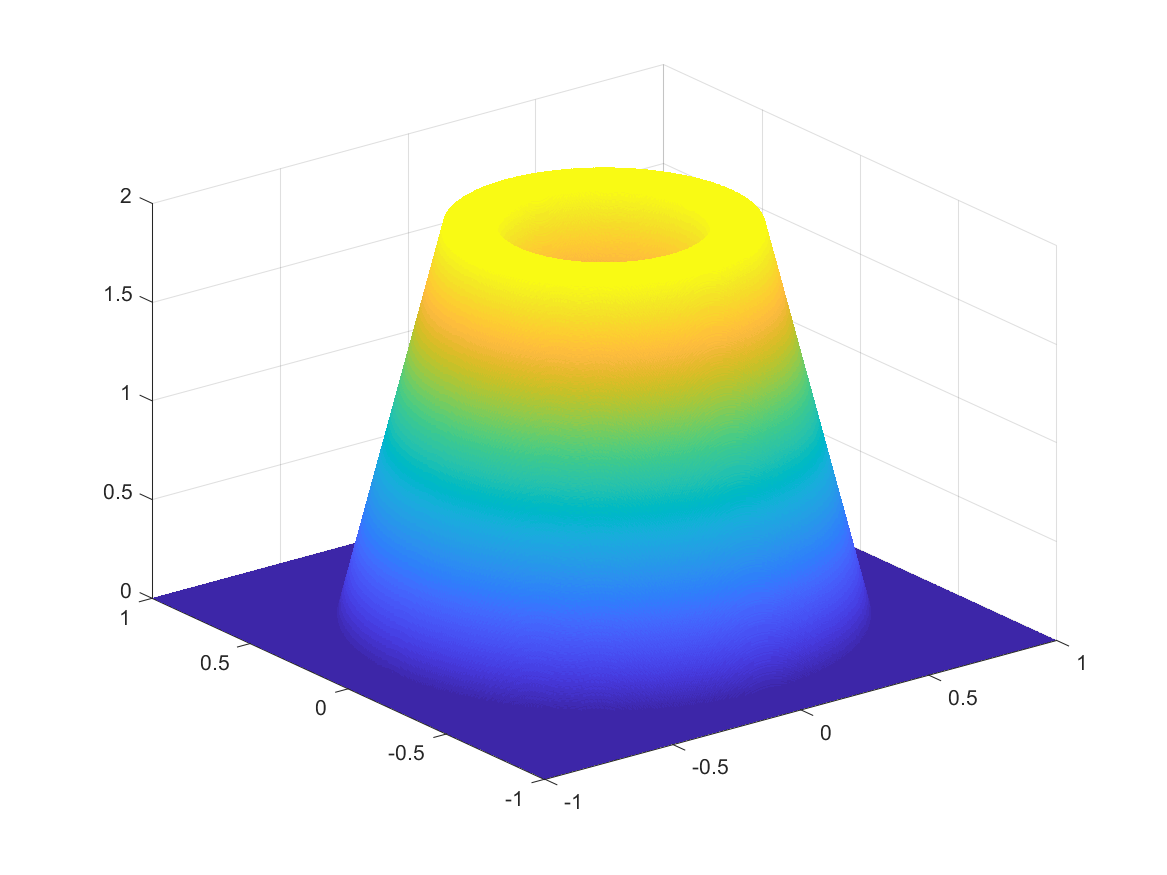
\includegraphics[trim = 40 30 30 30, clip, width=\linewidth]
      {pictures/chapExperiments/secGeneralInfo/f01Plots/exactSolution.png}
    \label{fig:f01ExactSol}
  \end{subfigure}
  \quad
  \begin{subfigure}[b]{.48\linewidth}
    \centering
    \caption{$u$ entlang der x- und y-Achse}
    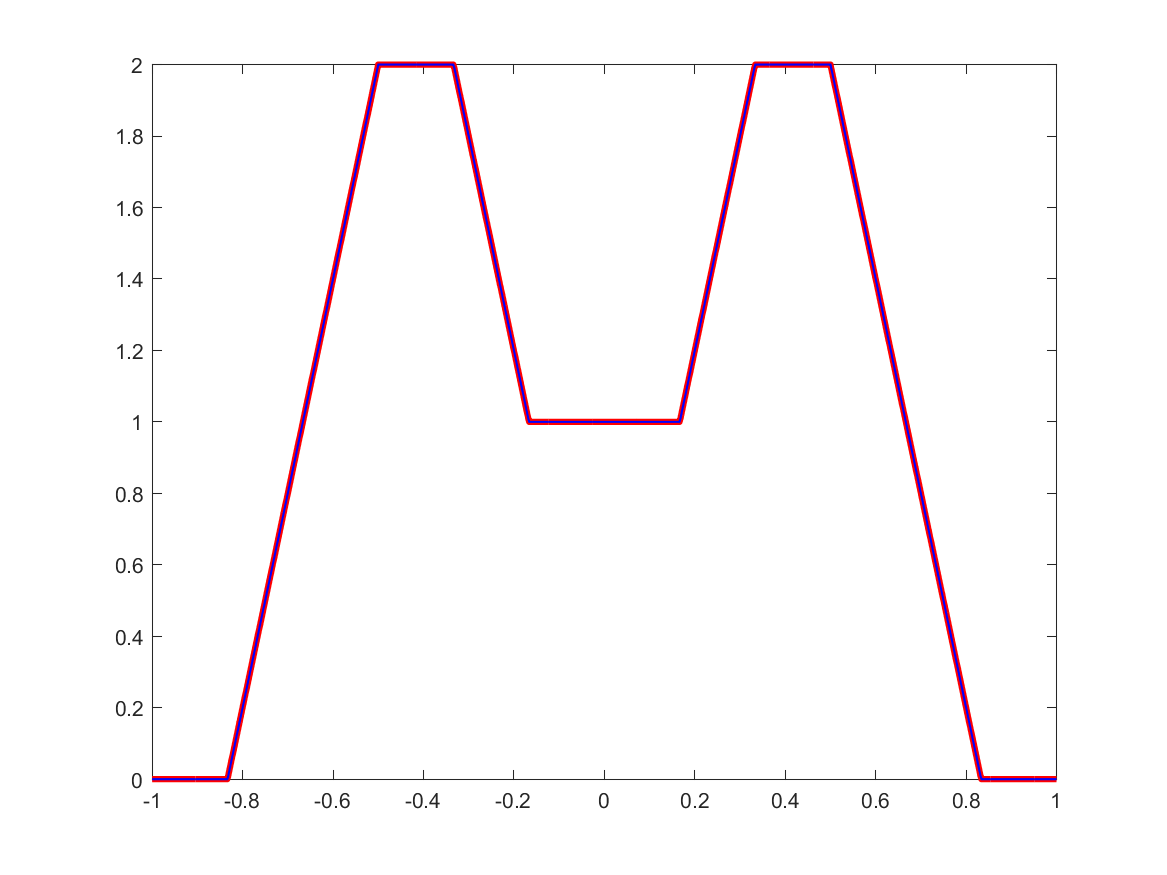
\includegraphics[trim = 50 30 50 20, clip, width=\linewidth]
      {pictures/chapExperiments/secGeneralInfo/f01Plots/exactSolutionAxis.png}
    \label{fig:f01ExactSolAxis}
  \end{subfigure} 
  \caption{Funktionen $f_\alpha$ und $u$ sowie deren
  Darstellungen entlang der x-Achse (blau) und der y-Achse (rot) für
  $\alpha\in\{1,10^4\}$}
  \label{fig:f01Plots}
\end{figure}
Die schwachen Gradienten von $u$ und $f_\alpha$ können bestimmt werden mithilfe
der partiellen Ableitungen
\begin{align*}
  \partial_r f_\alpha(r)
  &=
  \begin{cases}
    108,
    & \text{falls } r\in\left[0,\frac{1}{6}\right]\!,\\
    6\alpha\beta(6r-1)^{\beta-1} +\frac{1}{r^2}, 
    & \text{falls } r\in\left(\frac{1}{6},\frac{1}{3}\right]\!,\\
    \left(36\pi^2+\frac{1}{r^2}\right)\cos(\pi(6r-2))
    + \frac{6\pi}{r}\sin(\pi(6r-2)), 
    & \text{falls } r\in\left(\frac{1}{3},\frac{1}{2}\right]\!,\\
    -\left(6\alpha\beta\left( \frac{5}{2}-3r \right)^{\beta-1}+
    \frac{1}{r^2}\right),
    & \text{falls } r\in\left(\frac{1}{2},\frac{5}{6}\right]\!,\\
    -\left( \left( 18\pi^2+\frac{1}{2r^2} \right)\cos(\pi(6r-5))
    +\frac{1}{2r^2} + \frac{3\pi}{r}\sin(\pi(6r-5))\right)\!, 
    &\text{falls } r\in\left(\frac{5}{6},\infty\right)\!,
  \end{cases}
\end{align*}
und 
\begin{align*}
  \partial_r u(r) 
  &= 
  \begin{cases}
    0,
    & \text{falls } r\in\left[0,\frac{1}{6}\right]\!,\\
    6\beta(6r-1)^{\beta-1}, 
    & \text{falls } r\in\left(\frac{1}{6},\frac{1}{3}\right]\!,\\
    0, 
    & \text{falls } r\in\left(\frac{1}{3},\frac{1}{2}\right]\!,\\
    -6\beta\left( \frac{5}{2}-3r \right)^{\beta-1},
    & \text{falls } r\in\left(\frac{1}{2},\frac{5}{6}\right]\!,\\
    0,
    &\text{falls } r\in\left(\frac{5}{6},\infty\right)\!.
  \end{cases}
\end{align*} 
Durch Kenntnis des schwachen Gradienten von $u$ erhalten wir für das Experiment
mit Eingangssignal $f_\alpha$ die Approximation $E(u)\approx -2.05803$ für
$\alpha=1$ und $E(u)\approx -20\,580.34076$ für $\alpha=10^4$.
Ein weiteres Eingangssignal, welches wir in mehreren der folgenden Abschnitte
nutzen werden, ist das Graufarbenbild \texttt{cameraman} aus
\cref{fig:cameraman}, aus dem nach \Cref{rem:grayscalePictureInputSignal} ein
\texttt{function\_handle} erzeugt wird.


\section{Wahl der Parameter für die primale-duale Iteration}
\label{sec:choiceOfParameters}

Zunächst interessiert uns, wie der Parameter $\tau$ aus
\Cref{alg:primalDualIteration} gewählt werden sollte.
Durch \Cref{thm:convergenceIteration} ist uns bereits bekannt, dass
wir die Konvergenz der primalen-dualen Iteration nach ebendiesem Theorem nur 
für $\tau\in (0,1]$ garantieren können.
\begin{figure}[p]
  \centering
  \begin{subfigure}[b]{.48\linewidth}
    \caption{Eingangssignal $f_1$}
    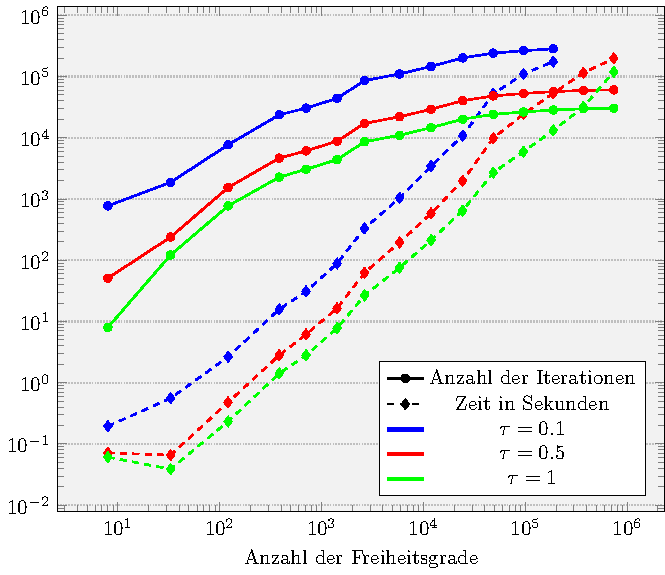
\includegraphics[width=\linewidth]
      {pictures/chapExperiments/secParameters/parTau/f01/miscF.pdf}
    \label{fig:parTauMiscF}
  \end{subfigure}
  \quad
  \begin{subfigure}[b]{.48\linewidth}
    \centering
    \caption{Eingangssignal \texttt{cameraman}}
    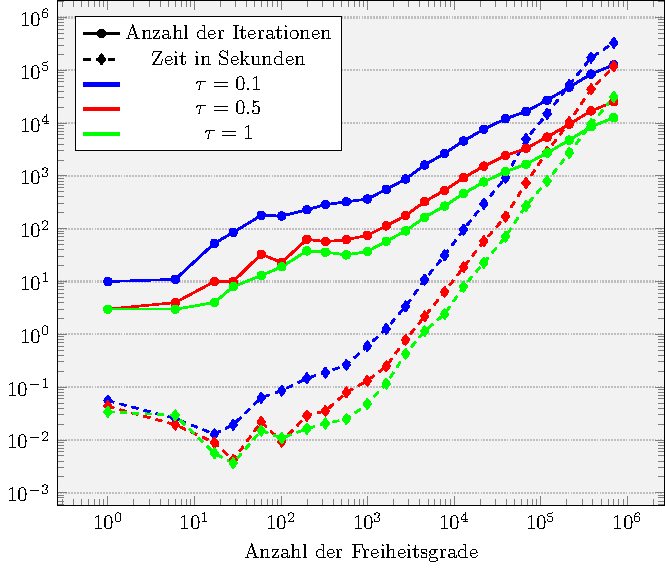
\includegraphics[width=\linewidth]
      {pictures/chapExperiments/secParameters/parTau/cam/miscCam.pdf}
    \label{fig:parTauMiscCam}
  \end{subfigure}
  \caption{Anzahl der Iterationen und benötigte Zeit für die primalen-dualen
    Iterationen während des AFEM-Algorithmus mit verschiedenen Werten von
    $\tau$ für die Eingangssignale $f_1$ und \texttt{cameraman}} 
  \label{fig:parTauMisc}
\end{figure}
In \Cref{fig:parTauMisc} sehen wir, dass die Anzahlen der Iterationschritte,
und damit auch die Laufzeiten, der primalen-dualen Iterationen während der
AFEM-Routine umso größer sind, je kleiner $\tau$ gewählt wird.
\begin{figure}[p]
  \centering
  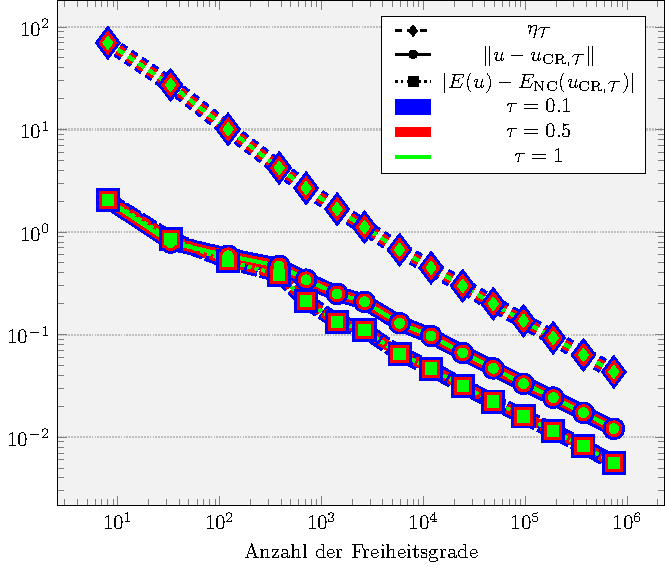
\includegraphics[width=.8\linewidth]
    {pictures/chapExperiments/secParameters/parTau/f01/convergenceF.pdf}
  \caption{Ergebnisse des Programms mit verschieden Werten von $\tau$ für das
    Eingangangssignal $f_1$}
  \label{fig:parTauConvergence}
\end{figure}
Da sich die betrachteten Graphen in \Cref{fig:parTauConvergence} für die
verschiedenen Wahlen von $\tau$ nicht sichtbar unterscheiden, vermuten wir,
dass die ideale Wahl für $\tau$ die maximale nach
\Cref{thm:convergenceIteration} zulässige ist.
Deshalb wählen wir für unsere Experimente $\tau=1$.
Ein mögliche Erklärung für unsere Beobachtung liefert der Beweis von
\Cref{thm:convergenceIteration}.
Die darin bewiesene Ungleichung \eqref{eq:upperBoundIterationError} impliziert
\begin{align}
  \label{eq:nrIterationsInequality}
  \sum_{j=1}^\infty\Vert \ucrt - \ujt \Vert^2 
  \leq
  \frac{1}{2\alpha\tau}
  \left(\vvvert \ucrt - u_{0,\Tcal}\vvvert^2_\nc 
  + \left\Vert \bar\Lambda_{0,\Tcal} - \Lambda_{0,\Tcal}\right\Vert^2\right)\!. 
\end{align}
Die rechte Seite ist antiproportional zu $\tau$, womit womöglich
die Folge $(\left\Vert \ucr - \ujt\right\Vert)_{j\in\Nbb}$ schneller gegen $0$
konvergiert und damit auch das Abbruchkriterium \eqref{eq:terminationCriterion}
nach einer geringeren Anzahl von Iterationen erfüllt ist. 
Allerdings schließt der Beweis von \Cref{thm:convergenceIteration} die
Konvergenz der primalen-dualen Iteration für $\tau>1$ nicht aus.
\begin{figure}[p]
  \centering
  \begin{subfigure}[b]{.48\linewidth}
    \centering
    \caption{Messungen der Updates}
    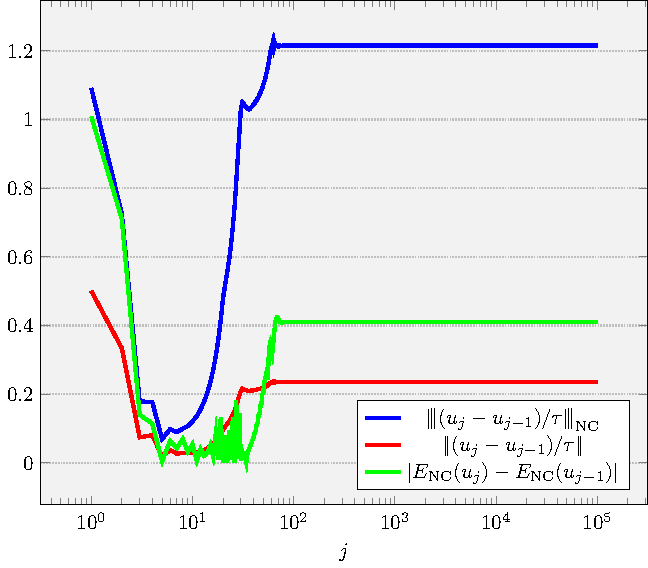
\includegraphics[width=\linewidth]
      {pictures/chapExperiments/secParameters/parTau/f01NoConv/1Dot2/convIter.pdf}
    \label{fig:parTauNoConvergenceUpdates}
  \end{subfigure}
  \quad
  \begin{subfigure}[b]{.47\linewidth}
    \centering
    \caption{Nichkonforme Energien}
    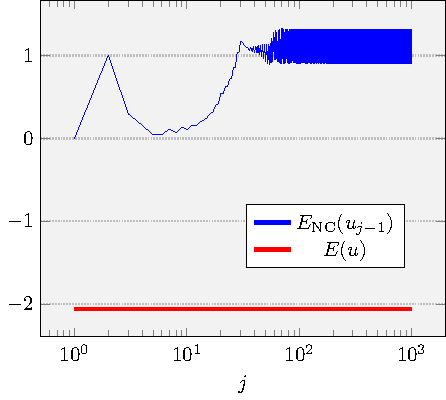
\includegraphics[width=\linewidth]
      {pictures/chapExperiments/secParameters/parTau/f01NoConv/1Dot2/convEnergy.pdf}
    \label{fig:parTauNoConvergenceEnergy}
  \end{subfigure}
  \caption{Verschiedene Messungen der Updates (a) und Verlauf der nichtkonformen
    Energien der ersten $1000$ Iterate (b) der primalen-dualen Iteration auf
    der Triangulierung \texttt{BigSquare} aus \Cref{fig:triangBigSquare} mit
    $\tau=1.2$ für das Eingangangssignal $f_1$}
  \label{fig:parTauNoConvergence}
\end{figure}
Wie aber in \Cref{fig:parTauNoConvergence} zu sehen, haben wir schon für
$\tau=1.2$ ein Beispiel gefunden, bei dem nicht davon ausgegangen werden kann,
dass die primale-duale Iteration konvergiert.
Dabei wurde die Iteration nach $10^5$ Schritten abgebrochen, da kein anderes
Verhalten mehr zu erwarten war.
Zusätzlich legitimiert wird der Abbruch nach $10^5$ Iterationen dadurch, dass
in \Cref{fig:parTauMiscF} auf der gleichen Triangulierung für die
suboptimale Wahl $\tau = 0.1$ weniger also $10^3$ Iterationen und für die Wahl
$\tau=1$ sogar weniger als $10$ Iterationen benötigt wurden.
Weiterhin zeigt \Cref{fig:parTauNoConvergenceUpdates}, dass auch für andere
Varianten, den Unterschied zweier aufeinanderfolgender Iterate im
Abbruchkriterium \eqref{eq:terminationCriterion} zu messen, die Iteration in
der Regel nicht abbricht.
Es scheint nach \Cref{fig:parTauNoConvergenceEnergy} außerdem festzustehen,
dass die nichtkonformen Energien der Iterate nach etwa $100$ Iterationen
oszillierend Werte annehmen.
Somit bleibt insgesamt festzuhalten, dass eine Konvergenzaussage im Wortlaut
von \Cref{thm:convergenceIteration} für $\tau\in(0,1.2]$ nicht mehr bewiesen
werden kann.

Als Nächstes begründen wir die Wahl $\epsstop = 10^{-4}$ für das
Abbruchkriterium \eqref{eq:terminationCriterion}.
\begin{figure}[p]
  \centering
  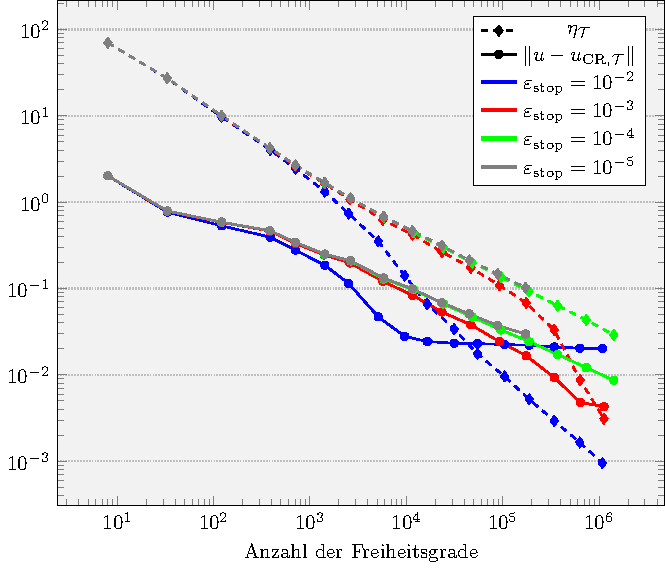
\includegraphics[width=.8\linewidth]
    {pictures/chapExperiments/secParameters/parEpsStop/f01/convergenceF.pdf}
  \caption{Ergebnisse des Programms mit verschieden Werten von $\epsstop$ für
    das Eingangangssignal $f_1$}
  \label{fig:parEpsStopConvergence}
\end{figure}
Wie in \Cref{fig:parEpsStopConvergence} zu sehen, stagniert der exakte
$L^2$-Fehler für $\epsstop=10^{-2}$ ab circa $10^4$ Freiheitsgraden und es
lässt sich erahnen, dass dieser Effekt auch für $\epsstop=10^{-3}$ ab ungefähr
$6\cdot 10^5$ Freiheitsgraden einsetzt.  
Dabei ist der erreichte Fehler für $\epsstop=10^{-3}$ geringer als
für $\epsstop=10^{-2}$.
Da für $\epsstop\in\{10^{-5},10^{-4}\}$ bis $10^6$ Freiheitsgrade dieses
Verhalten noch nicht zu sehen ist, scheint dies an einem zu frühen Abbruch der
Iteration durch eine zu große Wahl von $\epsstop$ zu liegen. 
Bei einer hohen Anzahl an Freiheitsgraden, das heißt bei kleinen Netzweiten,
muss also $\epsstop$ ausreichend klein sein, um die beobachtete Stagnation
des exakten Fehlers zu verhindern.
Da wir bei den Experimenten in dieser Arbeit $10^6$ Freiheitsgrade nicht
deutlich überschreiten und sich bis dahin die Ergebnisse für die Wahlen
$10^{-4}$ und $10^{-5}$ für $\epsstop$ in \Cref{fig:parEpsStopConvergence} kaum
unterscheiden, die Wahl $\epsstop=10^{-5}$ aber eine wesentlich längere
Laufzeit des Programms verursacht, begründen wir damit unsere Wahl
$\epsstop=10^{-4}$.
Allerdings bleibt anzumerken, dass der Verfeinerungsindikator $\etaT$ für alle
getesteten Wahlen von $\epsstop$ weiter fällt. 
Um dies zu untersuchen, betrachten wir die \Cref{def:refinementIndicator} von
$\etaT$.
Aus dieser folgt
\begin{align}
  \label{eq:etaEstimate}
  \etaT 
  \leq
  \max_{T\in\Tcal}|T|\Vert f-\alpha\ucrt\Vert^2
  + 2\max_{T\in\Tcal}|T|^{\gamma/2}\sum_{F\in\Ecal}\Vert[\ucrt]_F\Vert_{L^1(F)}.
\end{align}
Stagniert während der AFEM-Routine $\Vert u-\ucrt\Vert$, ist in Anbetracht
der Interpretation des ROF-Modells aus \Cref{chap:introduction} nicht
ausschließbar, dass $\Vert f-\alpha\ucrt\Vert^2$ ebenfalls stagniert.
Außerdem können wir nach den Überlegungen zu \Cref{fig:f01JumpTerms} in
\Cref{sec:experimentsWithExactSolution} davon ausgehen,
dass wahrscheinlich auch in den Experimenten aus
\Cref{fig:parEpsStopConvergence} die Terme
$\sum_{F\in\Ecal}\Vert[\ucrt]_F\Vert_{L^1(F)}$ im Verlauf des AFEM-Algorithmus
nicht gegen $0$ konvergieren.
Dennoch ist nach Ungleichung \eqref{eq:etaEstimate} die Konvergenz von $\etaT$
gegen $0$ weiterhin möglich, solange die Flächen der Dreicke $T\in\Tcal$
reduziert werden.  
Insbesondere kann davon ausgegangen werden, dass, nach Eintreten der 
beschriebenen Stagnation, der Flächeninhalt von Dreiecken beim Markieren durch 
$\etaT$ zunehmend wichtiger wird.
\begin{figure}[p]
  \centering
  \begin{subfigure}[b]{.48\linewidth}
    \centering
    \caption{$\epsstop=10^{-2}$}
    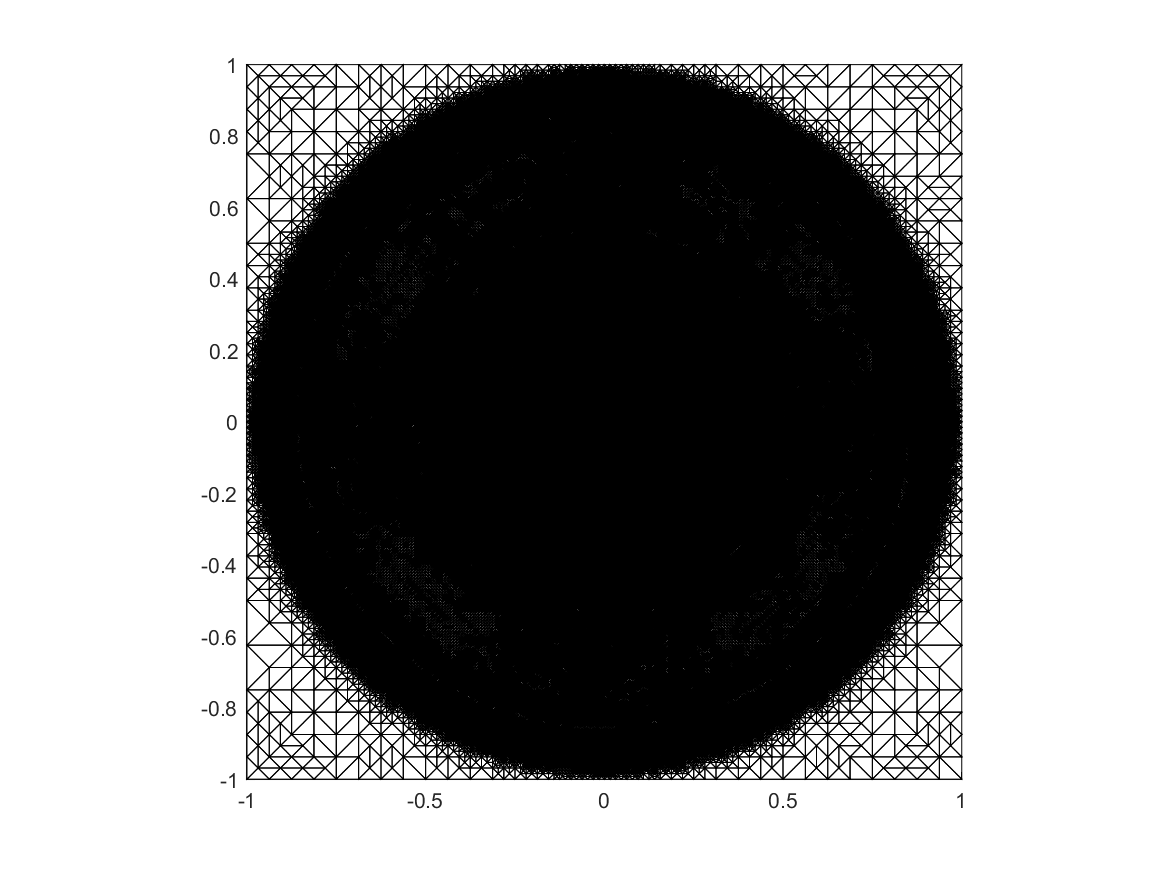
\includegraphics[trim = 100 30 80 20, clip, width=\linewidth]
      {pictures/chapExperiments/secParameters/parEpsStop/f01/1eM2/lvl15/triangulation.png}
    \label{fig:triangEpsStop1em2}
  \end{subfigure}
  \quad
  \begin{subfigure}[b]{.48\linewidth}
    \centering
    \caption{$\epsstop=10^{-5}$}
    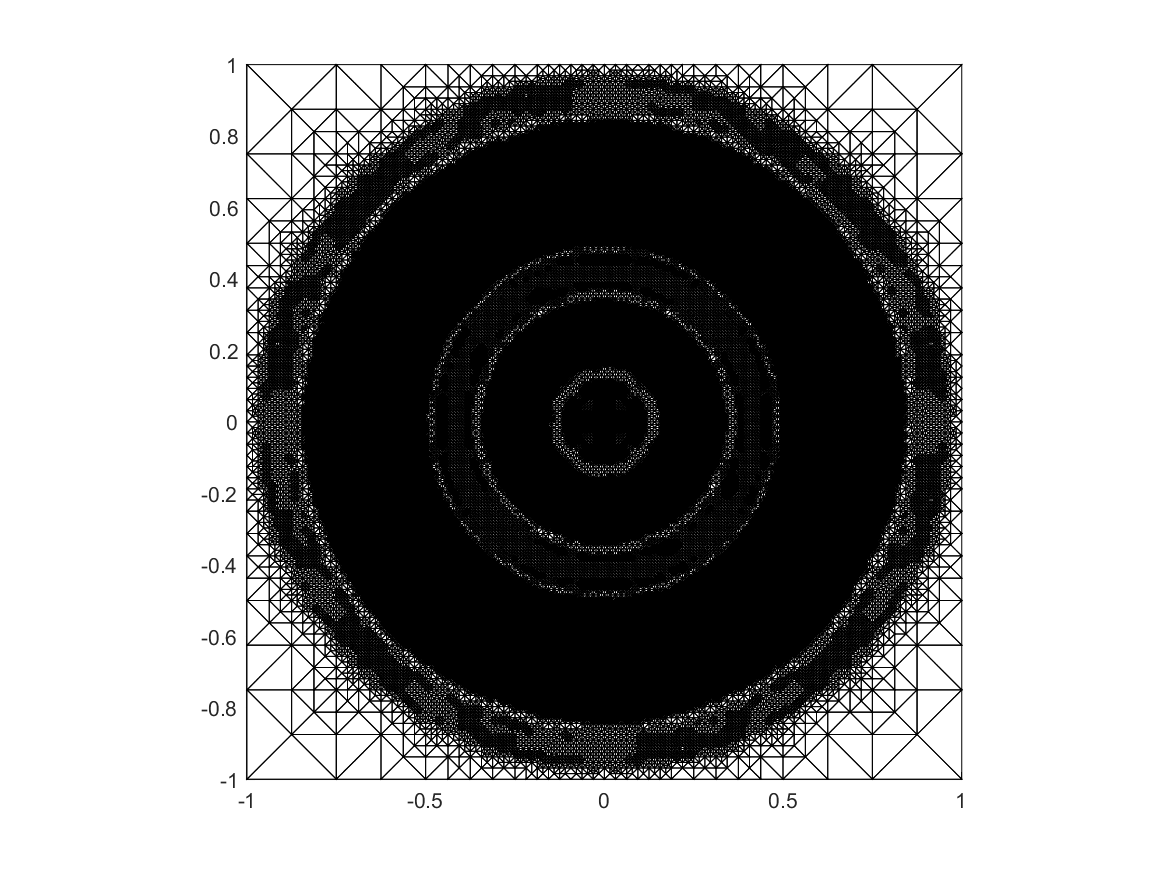
\includegraphics[trim = 100 30 80 20, clip, width=\linewidth]
      {pictures/chapExperiments/secParameters/parEpsStop/f01/1eM5/lvl14/triangulation.png}
    \label{fig:triangEpsStop1em5}
  \end{subfigure}
  \caption{Triangulierungen nach den Rechnungen mit verschiedenen Werten von
    $\epsstop$ nach jeweils circa 620\,000 Freiheitsgraden für das
    Eingangssignal $f_1$}
  \label{fig:triangEpsStop}
\end{figure}
Diese Vermutung scheint von \Cref{fig:triangEpsStop} gestützt zu werden, in der
wir sehen, dass bei einer vergleichbaren Anzahl von Freiheitsgraden der
abgebildeten Triangulierungen die Fläche des größten Dreiecks in
\Cref{fig:triangEpsStop1em2} zu $\epsstop=10^{-2}$ kleiner ist als die des
größten Dreiecks in \Cref{fig:triangEpsStop1em5} zu $\epsstop=10^{-5}$. 
Die vor Eintreten der Stagnation für $\epsstop\in\{10^{-3},10^{-2}\}$ im
Vergleich zu $\epsstop\in\{10^{-5},10^{-4}\}$ größere
Konvergenzgeschwindigkeit, die in \Cref{fig:parEpsStopConvergence} zu sehen
ist, lässt die Annahme zu, dass das Verfeinerung von Dreiecken mit großer
Fläche kurzzeitig eine effektive Strategie ist, insgesamt aber nicht zu
geringeren exakten Fehlern führt.


\section{Eigenschaften der primalen-dualen Iteration}
\label{sec:experimentsPrimalDualIteration}

Nun möchten wir anhand einiger Experimente mit Eingangssignal $f_1$ 
die primale-duale Iteration untersuchen.
\begin{figure}[p]
  \centering
  \begin{subfigure}[b]{.5\linewidth}
    \centering
    \caption{Nichtkonforme Energien der Iterate}
    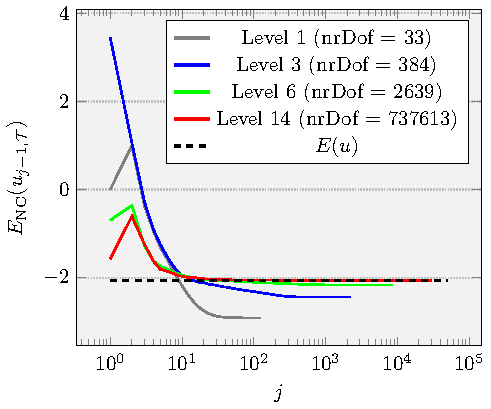
\includegraphics[width=\linewidth]
      {pictures/chapExperiments/secIterProps/lvlWise/convEnergy.pdf}
    \label{fig:iterationEnergyLevel}
  \end{subfigure}
  \quad
  \begin{subfigure}[b]{.46\linewidth}
    \centering
    \caption{Oszillierendes Beispiel}
    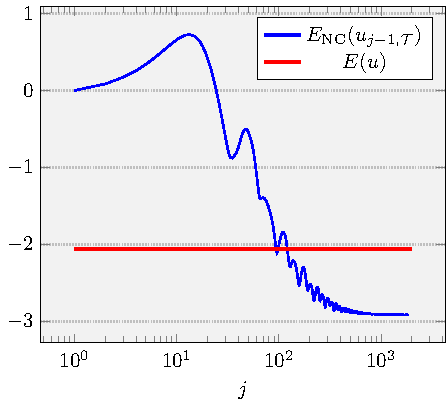
\includegraphics[width=\linewidth]
      {pictures/chapExperiments/secIterProps/osc/convEnergy.pdf}
    \label{fig:iterationEnergyOscillations}
  \end{subfigure}
  \caption{Entwicklung der nichtkonformen Energien der Iterate während der
    pri\-malen\--dualen Iteration auf verschiedenen Leveln der AFEM-Routine mit
    $\tau=1$ (a) und für ein Level mit 33 Freiheitsgraden und $\tau=10^{-1}$
    (b) für das Eingangssignal $f_1$}
  \label{fig:iterationEnergy}
\end{figure}
In \Cref{fig:iterationEnergyLevel} sehen wir an einer Auswahl von Leveln der
AFEM-Routine, dass die
nichtkonforme Energie $\Enc(\bullet)$ der Iterate von oben konvergiert. 
Dabei nimmt der Abstand des jeweiligen Grenzwerts zu der Energie der exakten
Lösung $E(u)$ mit zunehmender Anzahl von Freiheitsgraden ab.
Anhand des Ansteigens der nichtkonformen Energie im ersten Iterationsschritt
aller in \Cref{fig:iterationEnergyLevel} dargestellten Level, mit Ausnahme von
Level 3, ist aber auch klar erkennbar, dass die nichtkonformen Energien der
Iterate nicht monoton fallend konvergieren.
Dies können wir ebenfalls in \Cref{fig:iterationEnergyOscillations} sehen, in
der, auf einem Level mit 33 Freiheitsgraden für das gleiche Experiment mit
$\tau=10^{-1}$, die nichtkonformen Energien der Iterate oszillierend fallen.
Ebendieses Verhalten könnte ein Grund dafür sein, dass die  bis zum Abbruch der
primalen-dualen Iteration benötigte Anzahl an Iterationen für $\tau=10^{-1}$
deutlich höher ist als für $\tau=1$, wie wir bereits in \Cref{fig:parTauMiscF}
gesehen haben.
\begin{figure}[p]
  \centering
  \begin{subfigure}[b]{.5\linewidth}
    \centering
    \caption{Messungen der Updates}
    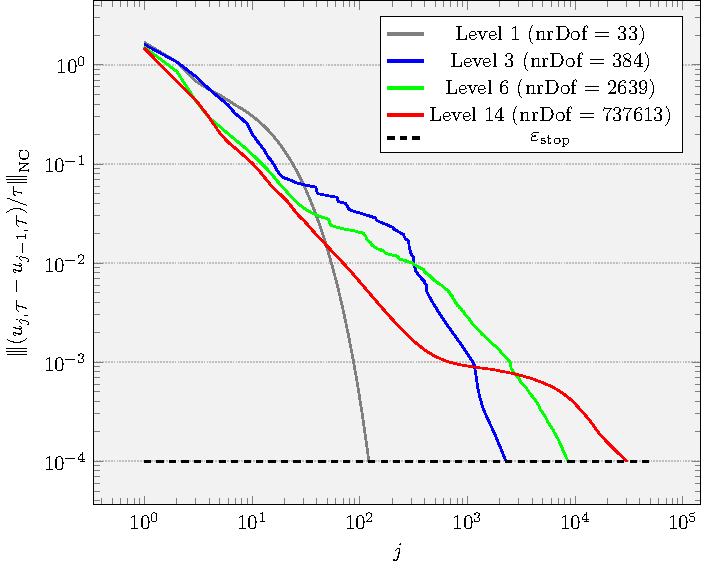
\includegraphics[width=\linewidth]
      {pictures/chapExperiments/secIterProps/lvlWise/termLvl.pdf}
    \label{fig:iterationLevel}
  \end{subfigure}
  \quad
  \begin{subfigure}[b]{.46\linewidth}
    \centering
    \caption{Varianten für die Messungen der Updates }
    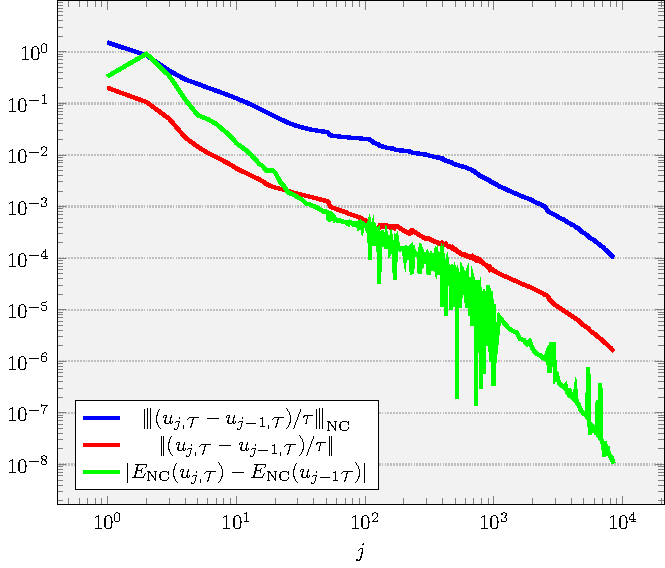
\includegraphics[width=\linewidth]
      {pictures/chapExperiments/secIterProps/lvlWise/termComp.pdf}
    \label{fig:iterationTerminationVariants}
  \end{subfigure}
  \caption{Verlauf der Messungen der Updates aus dem Abbruchkriterium 
    \eqref{eq:terminationCriterion} während der primalen-dualen Iteration auf
    verschiedenen Leveln der AFEM-Routine (a) und Verlauf von Varianten, diese
    Updates zu messen, für ein Level mit 2\,639 Freiheitsgraden (b) für das
    Eingangssignal $f_1$}
  \label{fig:iterationTermination}
\end{figure}
Als Nächstes betrachten wir \Cref{fig:iterationLevel}, in der die Entwicklung
der Messung des Unterschieds zweier aufeinanderfolgender Iterate im
Abbruchkriterium \eqref{eq:terminationCriterion} für verschiedene Level 
während der AFEM-Routine zu sehen ist.
Diese nimmt stets ohne Auffälligkeiten ab, bis sie den Wert $\epsstop$
erreicht.
Dabei ist wieder zu erkennen, dass die Anzahl der dazu benötigten Iterationen
mit steigender Anzahl an Freiheitsgraden zunimmt.
Zusätzlich sind in \Cref{fig:iterationTerminationVariants} für das sechste Level
derselben Rechnung die Verläufe zweier weiterer Varianten, 
den Unterschied von zwei aufeinanderfolgenden Iteraten zu messen, zu sehen.
Deren Konvergenz gegen $0$ ist zu erwarten, weshalb sie ebenfalls für das
Abbruchkriterium in Betracht gezogen werden könnten.
Dabei unterscheidet sich die Variante, bei der lediglich die $L^2$-Norm
anstelle der Energienorm verwendet wird, nur um einen Faktor von etwa
$10^2$ von der im Programm benutzten. 
Dies passt zur bekannten Theorie, da die Norm $\vvvert\bullet\vvvert_\NC$
ungefähr so skaliert wie $h^{-1}\Vert\bullet\Vert$ (cf. \cite[Lemma 3.5, Lemma
3.7]{Bar15}), wobei für das in \Cref{fig:iterationTerminationVariants} gezeigte
Level ungefähr gilt $h\approx 10^{-2}$.
Dementsprechend ist davon auszugehen, dass bei Wahl dieses Abbruchkriteriums 
nur die Toleranz $\epsstop$ angepasst werden müsste.
Die andere Variante zum Messen des Updates, das heißt der Betrag der Differenz
der nichtkonformen Energien zweier Iterate, scheint sich aber,
aufgrund der auftretenden Oszillationen, nur schlecht für ein 
Abbruchkriterium zu eignen.
Abschließend können wir festhalten, dass sich demnach das von uns gewählte 
Abbruchkriterium \eqref{eq:terminationCriterion} als sinnvoll erwiesen hat.

%\vfill

\section{Experimente mit bekannter exakter Lösung}
\label{sec:experimentsWithExactSolution}

In diesem Abschnitt möchten wir zunächst die Ergebnisse der Experimente mit
Eingangssignal $f_1$ bei adaptiver und uniformer Netzverfeinerung untersuchen
und einige Aussagen aus den theoretischen Kapiteln dieser Arbeit validieren.
\begin{figure}[p]
  \DTLloaddb{db}{data/currentDataReducedStandardF01LvlFinal.csv}
  \DTLassign{db}{1}{\nrDof=nrDof} 
  \DTLgdeletedb{db}
  \centering
  \begin{subfigure}[b]{.48\linewidth}
    \centering
    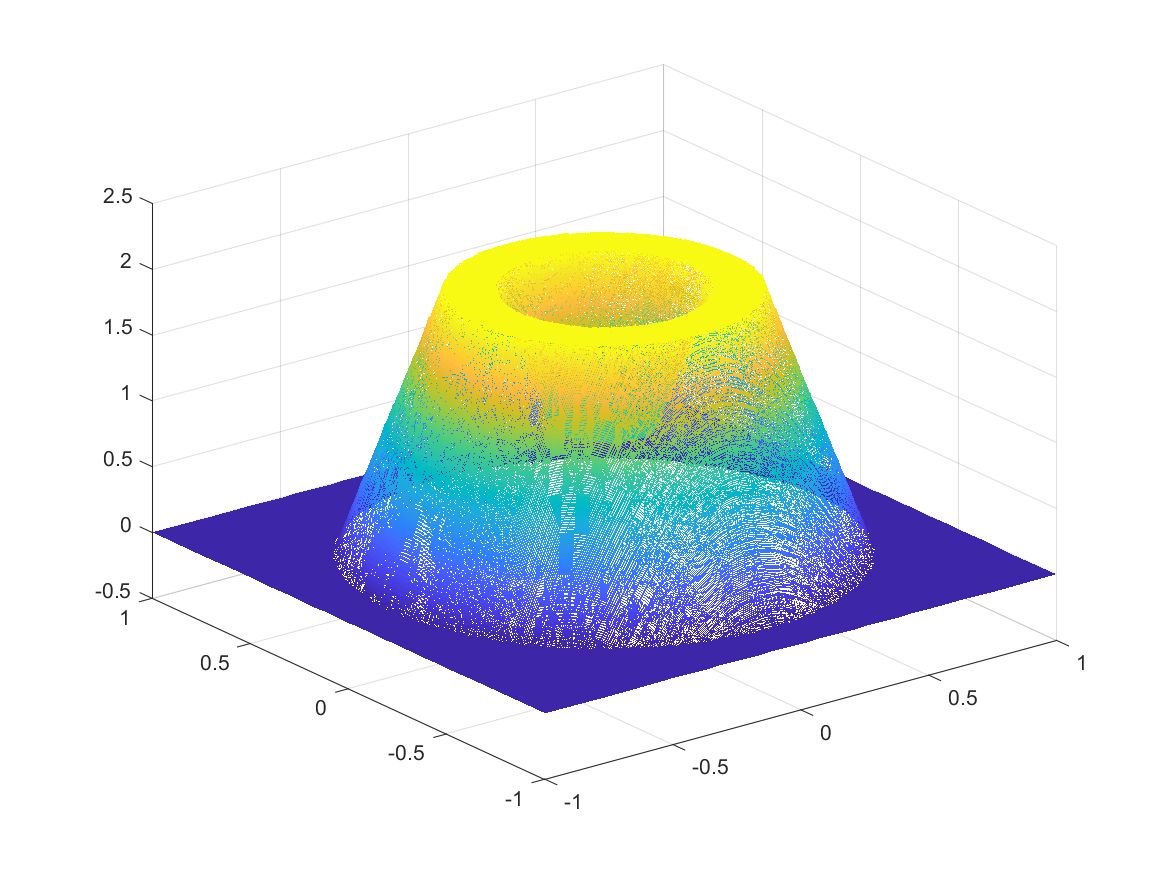
\includegraphics[trim = 40 30 30 30, clip, width=\linewidth]
      {pictures/chapExperiments/secExactSol/f01/adaptive/lvl14/solution.png}
    \label{fig:f01SolAdaptivePlot}
  \end{subfigure}
  \quad
  \begin{subfigure}[b]{.48\linewidth}
    \centering
    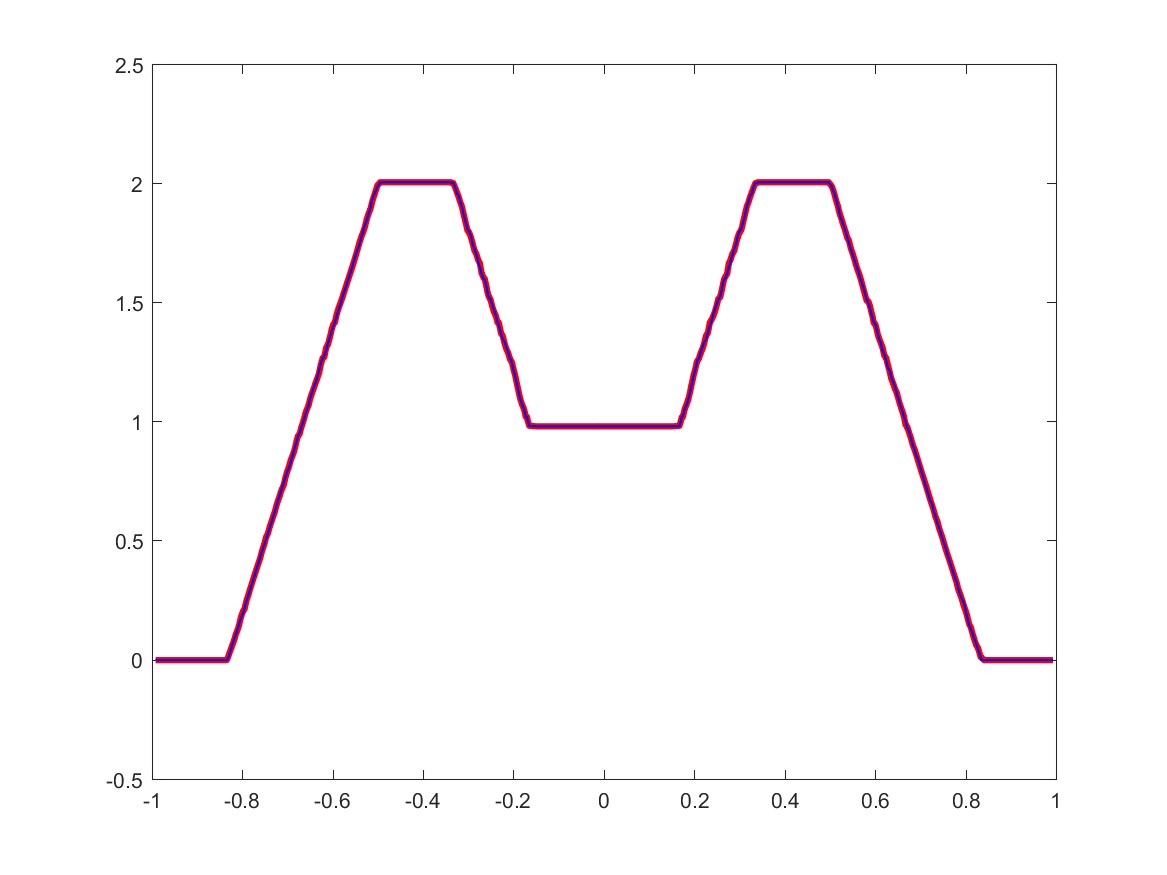
\includegraphics[trim = 50 30 50 20, clip, width=\linewidth]
      {pictures/chapExperiments/secExactSol/f01/adaptive/lvl14/solutionAxis.png}
    \label{fig:f01SolAdaptiveAxis}
  \end{subfigure}
  \caption{Lösung der Rechnung bei adaptiver Netzverfeinerung sowie deren
  Darstellungen entlang der x-Achse (blau) und der y-Achse (rot) nach etwa
  740\,000 Freiheitsgraden mit Eingangssignal $f_1$ }
  \label{fig:f01SolAdaptive}
\end{figure}
Die Lösung des Experiments mit adaptiver Netzverfeinerung ist in
\Cref{fig:f01SolAdaptive} dargestellt und ähnelt erkennbar der exakten Lösung
$u$ aus \Cref{fig:f01Plots}.
\begin{figure}[p]
  \centering
  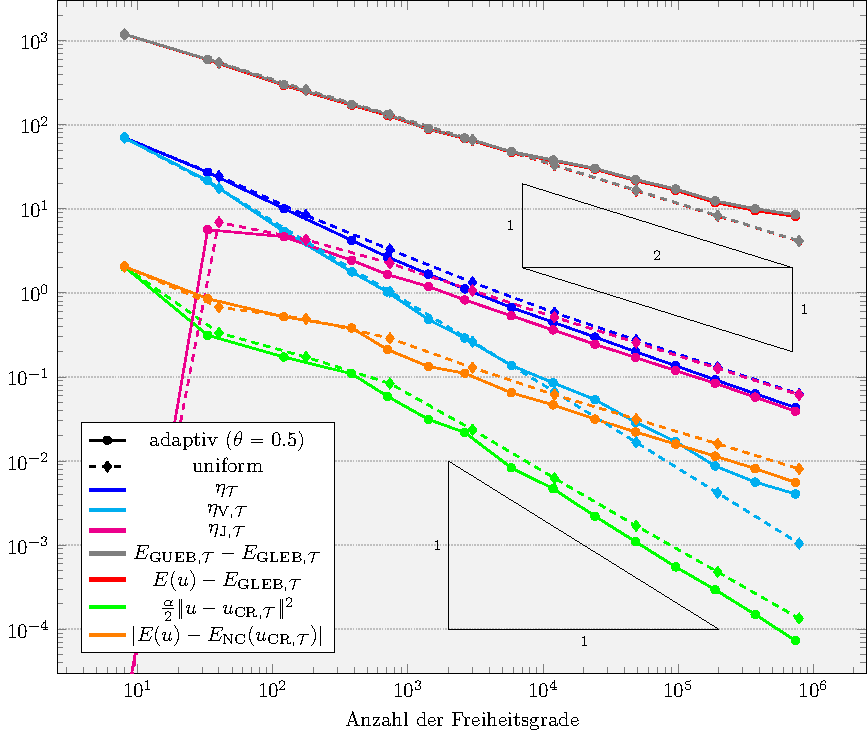
\includegraphics[width=.8\linewidth]
    {pictures/chapExperiments/secExactSol/f01/conv.pdf}
  \caption{Ergebnisse der Rechnungen mit adaptiver und uniformer 
    Netzverfeinerung für das Eingangssignal $f_1$}
  \label{fig:f01Convergence}
\end{figure}
Wie in \Cref{fig:f01Convergence} zu sehen, unterscheiden sich die
Konvergenzraten bei uniformer und adaptiver Netzverfeinerungen nur für den
Anteil $\etaV$ des Verfeinerungsindikators aus \Cref{def:refinementIndicator}
und für die Differenzen $\Egueb-\Egleb$ sowie $E(u)-\Egleb$ mit den
garantierten oberen und unteren Energieschranken $\Egueb$ und $\Egleb$ aus
\Cref{sec:refinementIndicatorAndGuaranteedBounds}.
Dabei können die Ratenunterschiede für diese Differenzen auf die für $\etaV$
zurückgeführt werden, denn nach Definition von $\Egleb$ in \Cref{eq:gleb}
und von $\etaV$ ist zu erwarten, dass der Wert von $\Egleb$ umso kleiner
ist, je größer der Wert von $\etaV$ ist. 
Tatsächlich nimmt in \Cref{fig:f01Convergence} bei adaptiver Netzverfeinerung 
$\etaV$ größere Werte an als bei uniformer, weshalb sich die beiden Graphen, in
denen $\Egleb$ subtrahiert wird, ebenso verhalten.
Die Konvergenzrate von $\etaV$ ist bei uniformer Netzverfeinerung etwa $1$ und
scheint bei adaptiver Netzverfeinerung kleiner als $1$ aber womöglich
größer als 1/2 zu sein.  
Allerdings wirken sich diese Ratenunterschiede von $\etaV$ bei adaptiver und
uniformer Netzverfeinerung nicht auf den Verfeinerungsindikator $\etaT$ aus,
denn dieser wird mit zunehmenden Freiheitsgraden deutlich von seinem Anteil
$\etaJ$ dominiert.
Damit hat $\etaT$, ebenso wie $\etaJ$, die Rate 1/2.

Durch \Cref{fig:iterationEnergyLevel} war bereits zu vermuten, dass die
nichtkonformen Energien der diskreten Lösungen $\Enc(\ucrt)$ gegen die Energie 
der exakten Lösung $E(u)$ konvergiert.
Nun sehen wir, dass $|E(u)-\Enc(\ucrt)|$ tatsächlich konvergiert mit einer 
Rate von etwa 1/2.
Weiterhin erwarten wir nach der Herleitung des diskreten Problems in
\Cref{sec:discreteProblemFormulation}, dass $E(\ucrt)$, im Gegensatz zu
$\Enc(\ucrt)$, nicht gegen $E(u)$ konvergiert.
\begin{figure}[p]
  \centering
  \begin{subfigure}[b]{.48\linewidth}
    \centering
    \caption{Entwicklung der Sprungterme}
    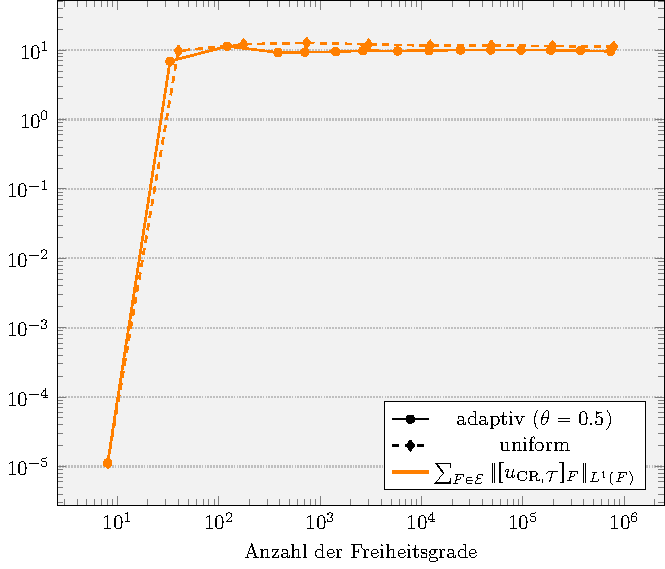
\includegraphics[width=\linewidth]
      {pictures/chapExperiments/secExactSol/f01/jumpTerms.pdf}
    \label{fig:f01JumpTerms}
  \end{subfigure}
  \quad
  \begin{subfigure}[b]{.48\linewidth}
    \centering
    \caption{Entwicklung der Energieschranken}
    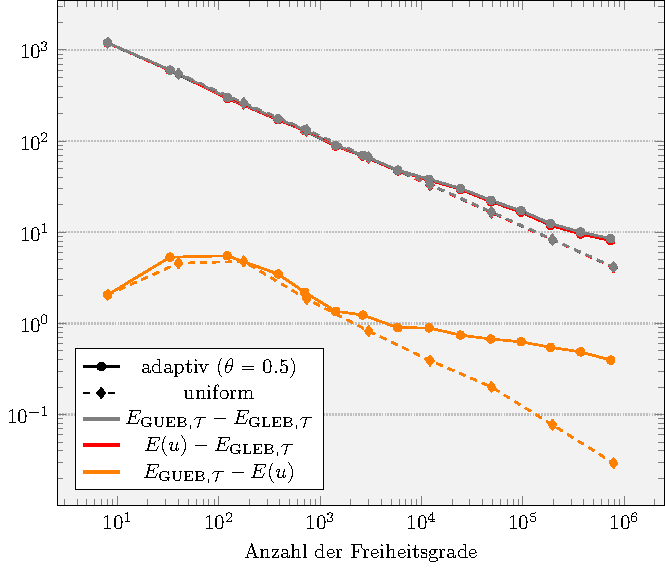
\includegraphics[width=\linewidth]
      {pictures/chapExperiments/secExactSol/f01/energyDiffs.pdf}
    \label{fig:f01DiffGuebExactE}
  \end{subfigure}
  \caption{Zusätzliche Ergebnisse der Rechnungen mit adaptiver und uniformer 
    Netzverfeinerung für das Eingangssignal $f_1$}
  \label{fig:f01SupplementaryInfo}
\end{figure}
Dies wird experimentell bestätigt durch \Cref{fig:f01JumpTerms}, in der wir
sehen, dass in unserer nichtkonformen Formulierung \Cref{prob:discreteProblem}
der Term $\sum_{F\in\Ecal}\Vert[\ucrt]_F\Vert_{L^1(F)}=E(\ucrt)-\Enc(\ucrt)$
tatsächlich nicht minimiert wird. 
Zwar sind die jeweiligen Sprünge zwischen zwei Dreiecken bei einer hohen Anzahl
von Freiheitsgraden klein, wie \Cref{fig:f01SolAdaptive} erahnen lässt, jedoch
führt eine hohe Anzahl an Kanten zur Addition von vielen Sprüngen und scheint
somit die Minimierung dieser Summe zu verhindern.
Außerdem wollen wir anmerken, dass aus \Cref{thm:convexity} und
\Cref{sec:discreteProblemFormulation} folgt, dass
\begin{align*}
  \frac{\alpha}{2}\Vert u-\ucrt\Vert^2
  \leq
  \left|\Enc(\ucrt)-E(u)\right|+
  \sum_{F\in\Ecal}\Vert[\ucrt]_F\Vert_{L^1(F)}.
\end{align*}
Nach \Cref{fig:f01Convergence} gilt sogar die Aussage $\frac{\alpha}{2}\Vert
u-\ucrt\Vert^2 \leq \left|\Enc(\ucrt)-E(u)\right|$, obwohl
$\sum_{F\in\Ecal}\Vert[\ucrt]_F\Vert_{L^1(F)}$ nicht minimiert wird.

Die Graphen von $\Egueb-\Egleb$ sowie von $E(u)-\Egleb$ zeigen bei uniformer
Netzverfeinerung die Konvergenzrate $1/2$ und bei adaptiver Netzverfeinerung, wie
bereits begründet, eine etwas geringere.
Dabei gilt stets
\begin{align}
  \label{eq:expectedInequalities}
  \frac{\alpha}{2}\Vert u -\ucrt\Vert^2
  \leq
  E(u)-\Egleb
  \leq
  \Egueb-\Egleb,
\end{align}
wie wir nach \Cref{thm:gleb} und Ungleichung \ref{eq:gueb} erwartet haben.
Die Gültigkeit der zweiten Ungleichung in \eqref{eq:expectedInequalities}
können wir deutlich an der Differenz $\Egueb-E(u)$ von $\Egueb-\Egleb$ und
$E(u)-\Egleb$ erkennen, die in \Cref{fig:f01DiffGuebExactE} dargestellt ist.
Dabei konvergiert der quadrierte exakte Fehler $\frac{\alpha}{2}\Vert
u-\ucrt\Vert^2$ mit Rate 1.
Nach \cite[S. 309, Theorem 10.7]{Bar15} ist für das dort betrachtete Problem,
das heißt der Diskretisierung des ROF-Modells mit dem
Courant-Finite-Elemente-Raum $S^1(\Tcal)$ für ein Eingangssignal $g\in
L^\infty(\Omega)$, für den quadrierten $L^2$-Fehler zwischen den Minimierern
$u_\C\in S^1(\Tcal)$ und $u\in\BV(\Omega)\cap L^2(\Omega)$ des Funktionals $I$
aus \Cref{eq:rofModel} in den entsprechenden Räumen eine Rate von 1/4
garantiert.
Obwohl wir eine alternative Formulierung des ROF-Modells betrachten und diese
mit dem Crouzeix-Raviart-Finite-Elemente-Raum diskretisieren, können wir
festhalten, dass die hier beobachtete Konvergenzrate für $\frac{\alpha}{2}\Vert
u-\ucrt\Vert^2$ deutlich besser ist.
Dabei bleibt aber noch hervorzuheben, dass für das Experiment in
\Cref{fig:f01Convergence} gilt $u,f_1\in H^1_0\left( (0,1)^2 \right)$. 
Insbesondere ist unsere exakte Lösung sogar schwach differenzierbar und nicht
nur eine Funktion von beschränkter Variation, weshalb die bessere Rate 
nicht unerwartet ist.
Um ein anderes Eingangssignal für ein Experiment mit bekannter exakter Lösung
zu betrachten und dabei zu untersuchen, ob noch stärkere Annahmen an die
schwache Differenzierbarkeit der exakten Lösung und des Eingangssignals die
Raten weiter verbesser können, betrachten wir nun die Funktion
$u_\textrm{HR} \in H^2_0\left((0,1)^2\right)$, die gegeben ist durch 
\begin{align*}
  u_\textrm{HR}(r)\coloneqq 
  \begin{cases}
    1, 
    & \text{falls } r\in\left[0, \frac{1}{3}\right]\!,\\
    54r^3 - 81r^2 + 36r - 4, 
    & \text{falls } r\in\left(\frac{1}{3}, \frac{2}{3}\right]\!,\\
    0, 
    & \text{falls } r\in\left(\frac{2}{3}, \infty\right)\!.
  \end{cases}
\end{align*}
Mit der Wahl
\begin{align*}
  \sgn&(\partial_r u_\textrm{HR}(r)) 
  \coloneqq 
  \begin{cases}
    -1458r^5 + 1215r^4 - 270r^3, 
    & \text{falls } r\in\left[0, \frac{1}{3}\right]\!,\\
    -1,
    & \text{falls } r\in\left(\frac{1}{3}, \frac{2}{3}\right]\!,\\
    -243r^4 + 756r^3 - 864r^2 + 432r - 81, 
    & \text{falls } r\in\left(\frac{2}{3}, \infty\right)\!,
  \end{cases}
\end{align*}
ist $u_\textup{HR}$ die exakte Lösung von \Cref{prob:continuousProblem} mit
Eingangssignal
\begin{align*}
  f_\textrm{HR}(r)\coloneqq 
  \begin{cases}
    \alpha + 8748r^4 - 6075r^3 + 1080r^2, 
    & \text{falls } r\in\left[0, \frac{1}{3}\right]\!,\\
    \alpha\left(54r^3 - 81r^2 + 36r - 4\right) + \frac{1}{r}, 
    & \text{falls } r\in\left(\frac{1}{3}, \frac{2}{3}\right]\!,\\
    1215r^3 - 3024r^2 + 2592r - 864 + \frac{81}{r}, 
    & \text{falls } r\in\left(\frac{2}{3}, \infty\right)\!,
  \end{cases}
\end{align*}
für das ebenfalls gilt $f_\textrm{HR}\in H^2_0\left((0,1)^2\right)$.
Die schwachen Ableitungen können wieder berechnet werden durch 
die partiellen Ableitungen
\begin{align*}
  \partial_r f_\textrm{HR}(r) =
  \begin{cases}
    34992r^3 - 18225r^2 + 2160r, 
    & \text{falls } r\in\left[0, \frac{1}{3}\right]\!,\\
    \alpha\left(162r^2 - 162r + 36\right) - \frac{1}{r^2}, 
    & \text{falls } r\in\left(\frac{1}{3}, \frac{2}{3}\right]\!,\\
    3645r^2 - 6048r + 2592 - 864 - \frac{81}{r^2}, 
    & \text{falls } r\in\left(\frac{2}{3}, \infty\right)\!,
  \end{cases}
\end{align*}
und
\begin{align*}
  \partial_r u_\textrm{HR}(r) &=
  \begin{cases}
    0,
    & \text{falls } r\in\left[0, \frac{1}{3}\right]\!,\\
    162r^2 - 162r + 36, 
    & \text{falls } r\in\left(\frac{1}{3}, \frac{2}{3}\right]\!,\\
    0, 
    & \text{falls } r\in\left(\frac{2}{3}, \infty\right)\!.
  \end{cases}
\end{align*}
Wir wählen für das Experiment $\alpha=1$ und erhalten für die Energie 
der exakten Lösung $E(u_\textup{HR})\approx -0.33411$.
\begin{figure}[p]
  \centering
  \begin{subfigure}[b]{.38\linewidth}
    \centering
    \caption{$f_\textrm{HR}$}
    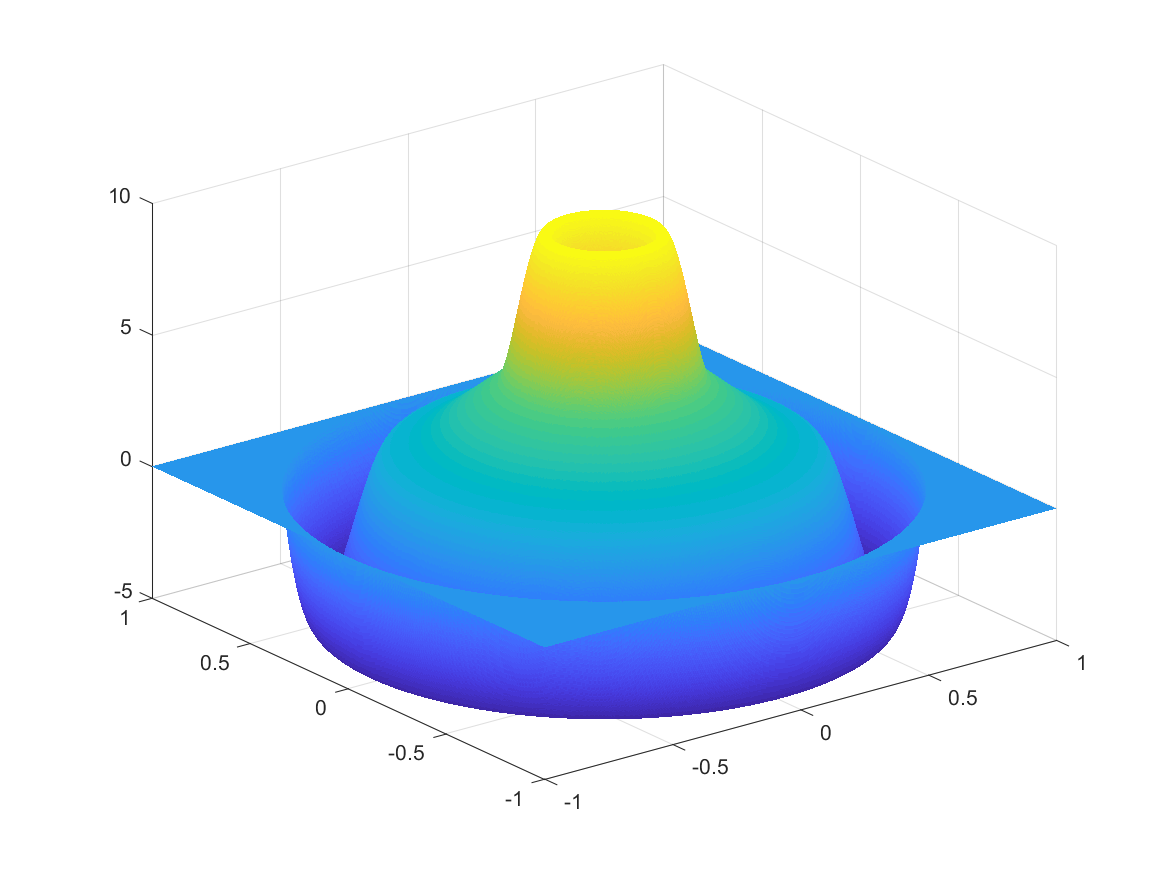
\includegraphics[trim = 40 30 30 30, clip, width=\linewidth]
      {pictures/chapExperiments/secExactSol/f04/inSi.png}
    \label{fig:f04InSi}
  \end{subfigure}
  \quad
  \begin{subfigure}[b]{.38\linewidth}
    \centering
    \caption{$f_\textrm{HR}$ entlang der x- und y-Achse}
    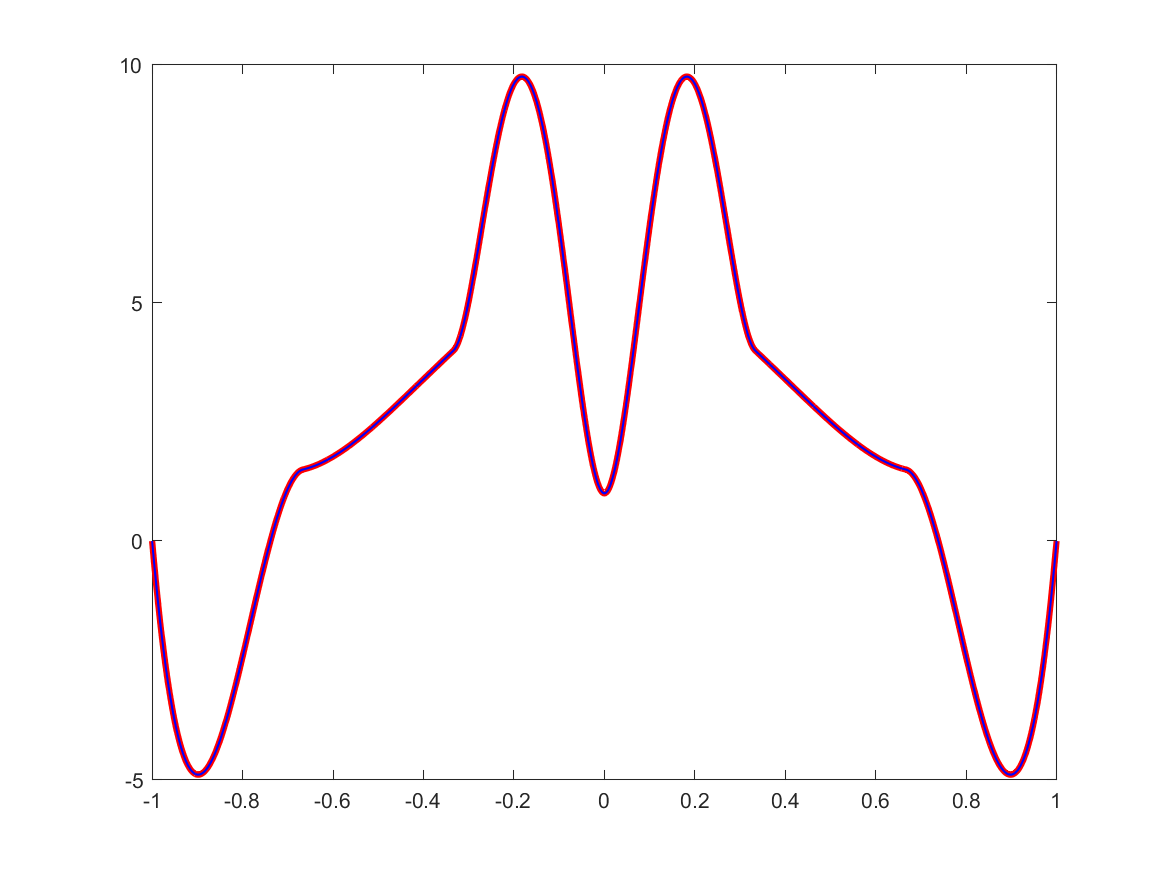
\includegraphics[trim = 50 30 50 20, clip, width=\linewidth]
      {pictures/chapExperiments/secExactSol/f04/inSiAxis.png}
    \label{fig:f04InSiAxis}
  \end{subfigure}

  \begin{subfigure}[b]{.38\linewidth}
    \centering
    \caption{$u_\textrm{HR}$}
    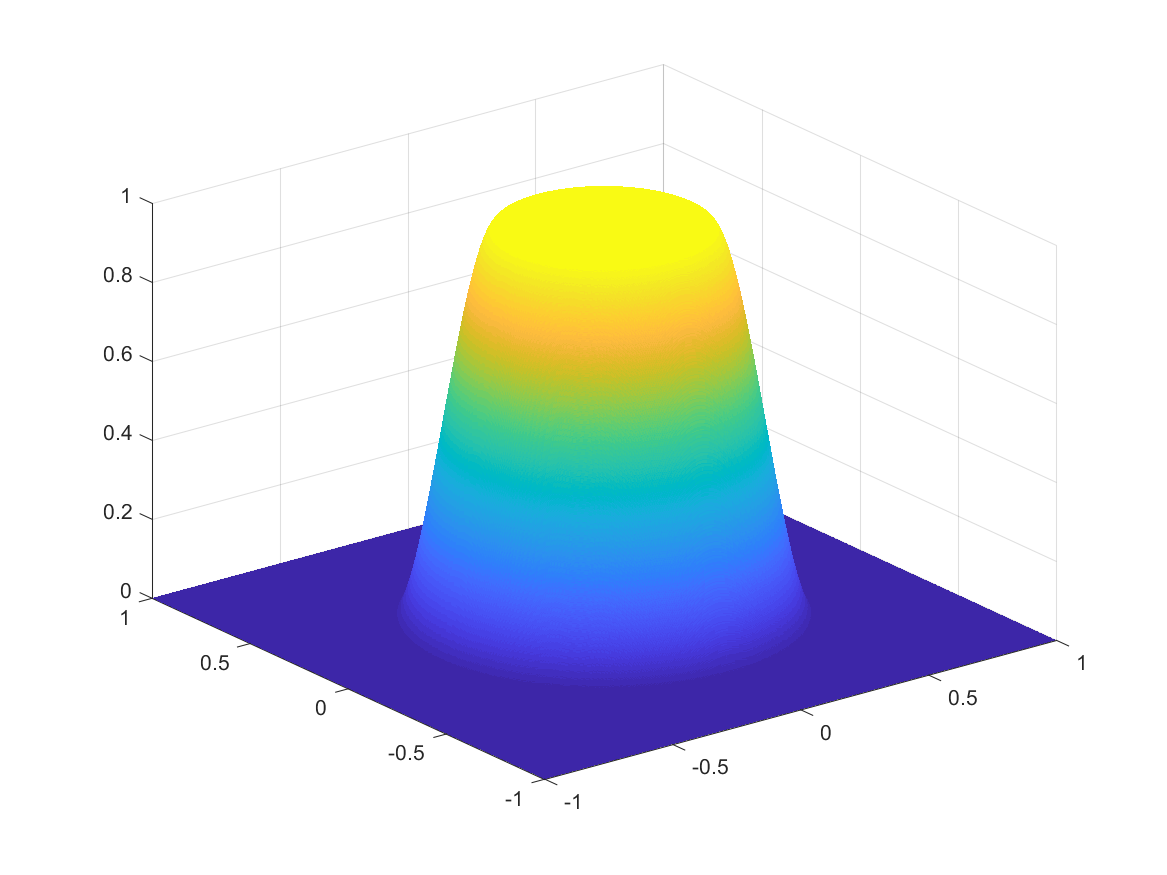
\includegraphics[trim = 40 30 30 30, clip, width=\linewidth]
      {pictures/chapExperiments/secExactSol/f04/exactSolution.png}
    \label{fig:f04ExactSol}
  \end{subfigure}
  \quad
  \begin{subfigure}[b]{.38\linewidth}
    \centering
    \caption{$u_\textrm{HR}$ entlang der x- und y-Achse}
    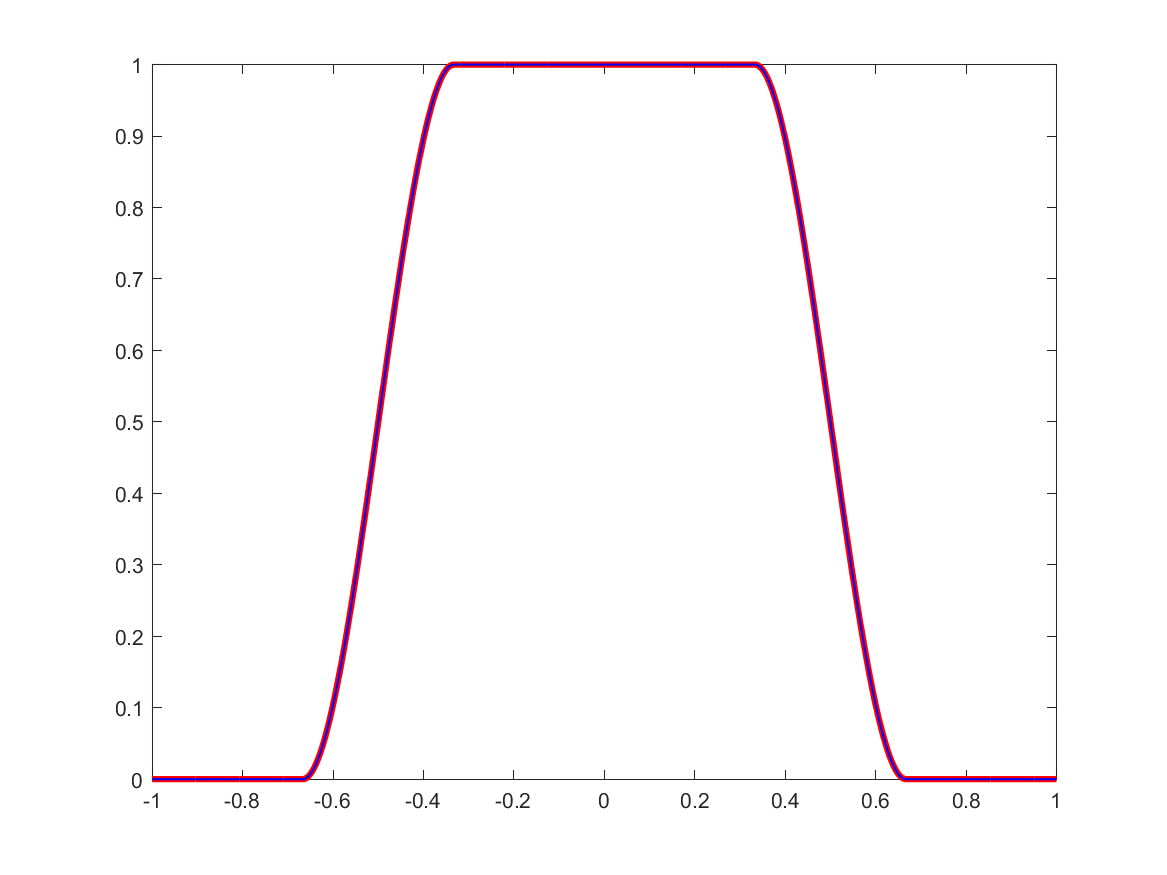
\includegraphics[trim = 50 30 50 20, clip, width=\linewidth]
      {pictures/chapExperiments/secExactSol/f04/exactSolutionAxis.png}
    \label{fig:f04ExactSolAxis}
  \end{subfigure} 
  \caption{Funktionen $f_\textrm{HR}$ und $u_\textup{HR}$ sowie deren
  Darstellungen entlang der x-Achse (blau) und der y-Achse (rot) für
  $\alpha = 1$}
  \label{fig:f04Plots}
\end{figure}
Dieses Eingangssignal und die exakte Lösung sind in \Cref{fig:f04Plots}
dargestellt.
\begin{figure}[p]
  \centering
  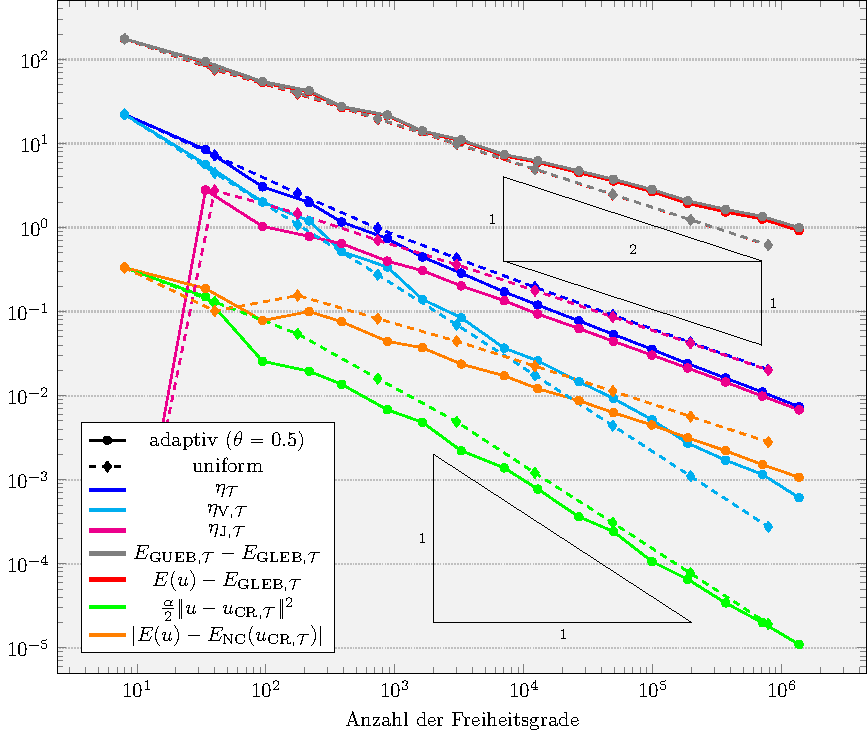
\includegraphics[width=.8\linewidth]
    {pictures/chapExperiments/secExactSol/f04/conv.pdf}
  \caption{Ergebnisse der Rechnungen mit adaptiver und uniformer 
    Netzverfeinerung für das Eingangssignal $f_\textup{HR}$}
  \label{fig:f04Convergence}
\end{figure}
Allerdings stellen wir in \Cref{fig:f04Convergence} lediglich fest, dass im
Vergleich zu \Cref{fig:f01Convergence} alle Graphen um einen Faktor von etwa
$10^{1/2}$ nach unten verschoben sind.
Insbesondere verändern sich die Konvergenzraten nicht.
Eine noch stärkere Regularitätsanname scheint die Raten also nicht weiter zu
verbessern, es werden aber geringfügig kleinere Werte erreicht.
Möglicherweise sind bei der hier benutzten Diskretisierung keine besseren Raten
erreichbar und die Betrachtung einer Methode höherer Ordnung wäre dazu
notwendig.

Nun betrachten wir noch einmal das Eingangssignal $f_1$, um den Einfluss der
Wahl von $\gamma\in(0,1]$ aus der \Cref{def:refinementIndicator} des
Verfeinerungsindikators $\etaT$ auf die Rechungen zu untersuchen.
Je kleiner die Wahl von $\gamma$, desto dominanter sollte nach Definition der
Einfluss von $\etaJ$ auf $\etaT$ sein und entsprechend dort stärker 
verfeinert werden, wo die Kantensprünge größer sind.
Dieser Effekt sollte auch für $\gamma=0$ zu beobachten sein, weshalb wir
diese Wahl ebenfalls untersuchen.
\begin{figure}[p]
  \centering
  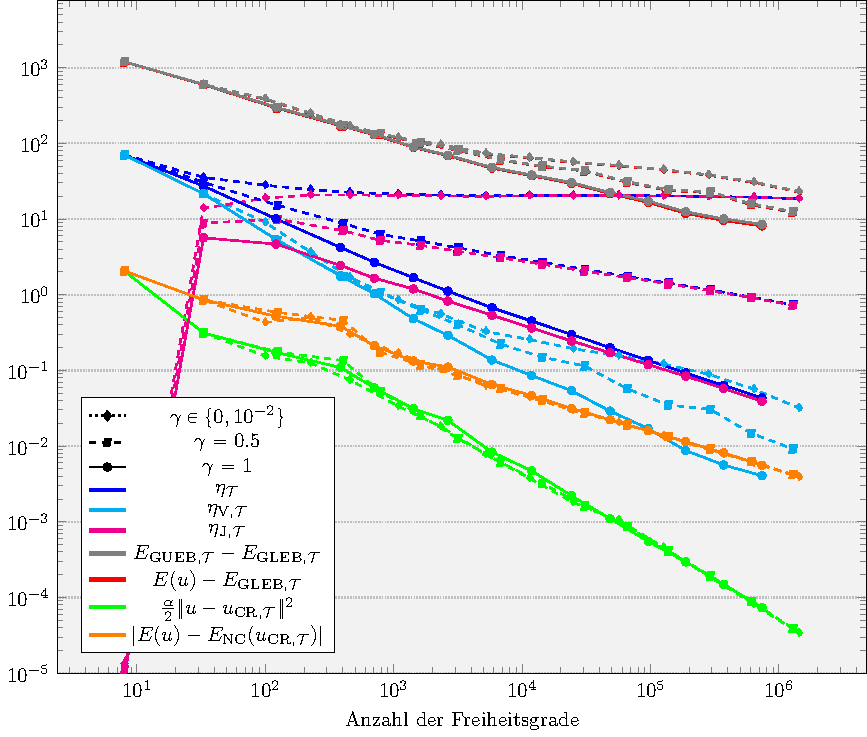
\includegraphics[width=.8\linewidth]
    {pictures/chapExperiments/secExactSol/parGamma/conv.pdf}
  \caption{Ergebnisse des Programms mit verschiedenen Werten von $\gamma$ für
    das Eingangssignal $f_1$, wobei die Graphen für $\gamma \in\{0,10^{-2}\}$
    nicht sichtbar unterscheidbar sind und deshalb nur der Graph für $\gamma=0$
    dargestellt ist}
  \label{fig:parGammaConvergence}
\end{figure}
In \Cref{fig:parGammaConvergence} ist tatsächlich zu erkennen, dass
$\etaJ$ mit kleinerem $\gamma$ deutlich größere Werte annimmt, sodass
sogar die Konvergenzrate von $\etaJ$ abnimmt. 
Da $\etaJ$ den Verfeinerungsindikator $\etaT$ dominiert, zeigt dieser das
gleiche Konvergenzverhalten.
Für $\gamma=0$ stagniert $\etaJ$ sogar.
Eine Erklärung für diese Beobachtungen ist, dass, wie bereits
festgestellt, die Sprungterme $\sum_{F\in\Ecal(\Tcal)}\Vert
[\ucrt]_F\Vert_{L^1(F)}$ nicht minimiert werden.
Insbesondere für $\gamma=0$ wird somit im Verfeinerungsindikator der Anteil
$\etaJ$ stark gewichtet, der in diesem Fall nicht gegen 0 konvergiert.  
Weiterhin ist die Konvergenzrate von $\etaV$ etwas schlechter, wenn $\gamma$
klein gewählt wird.
Die Fehlergraphen $\frac{\alpha}{2}\Vert u-\ucrt\Vert^2$ und
$|E(u)-\Enc(\ucrt)|$ zeigen allerdings für die verschiedenen Wahlen von
$\gamma$ keine nennenswerten Unterschiede. 
Die für den Verfeinerungsindikator suboptimalen Wahlen von $\gamma$ scheinen
also keinen negativen Effekt auf diese zu haben.
\begin{figure}[p]
  \centering
  \begin{subfigure}{.32\linewidth}
    \centering
    \caption{$\gamma=0$, $\text{nrDof}\approx 1\,440\,000 $}
    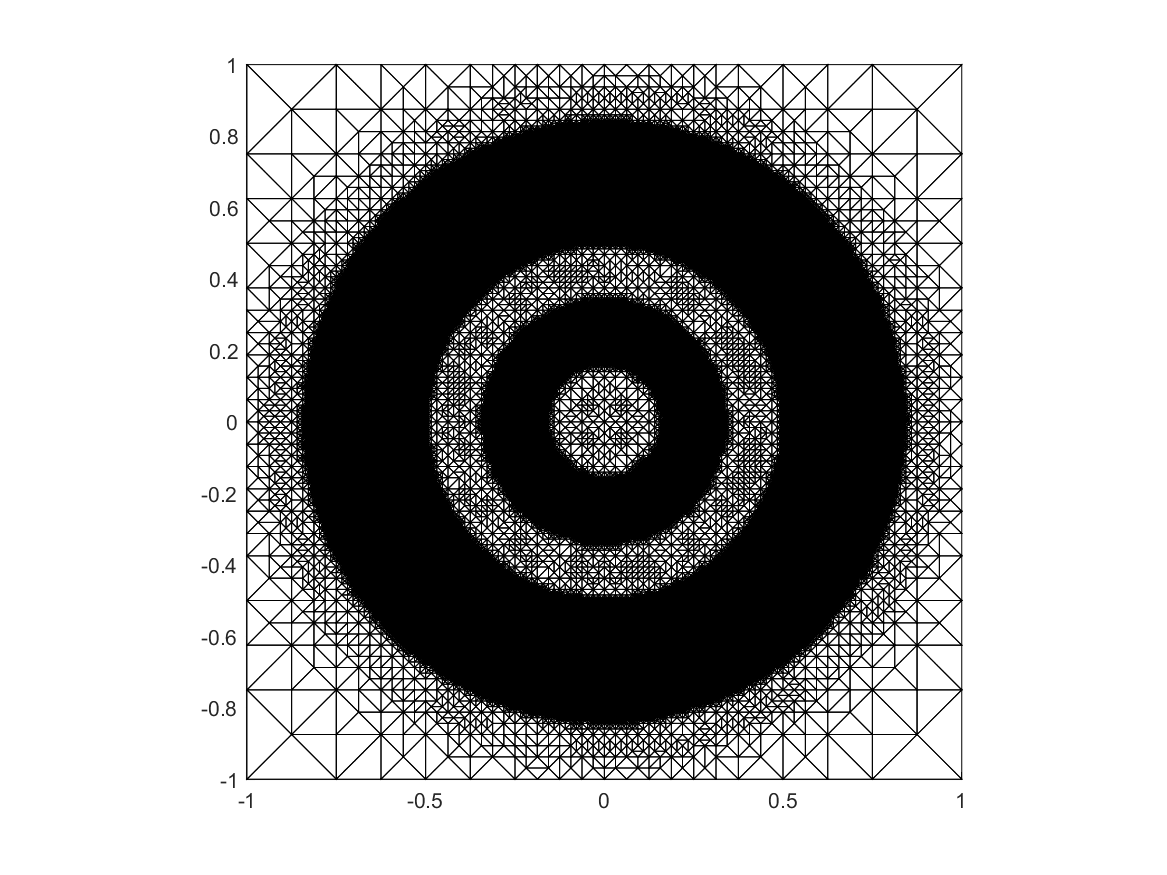
\includegraphics[trim = 100 30 80 20, clip, width=\linewidth]
      {pictures/chapExperiments/secExactSol/parGamma/0/lvl14/triangulation.png}
    \label{fig:gamma0Triang}
  \end{subfigure}
  \begin{subfigure}{.32\linewidth}
    \centering
    \caption{$\gamma=0.5$, $\text{nrDof}\approx 1\,280\,000$}
    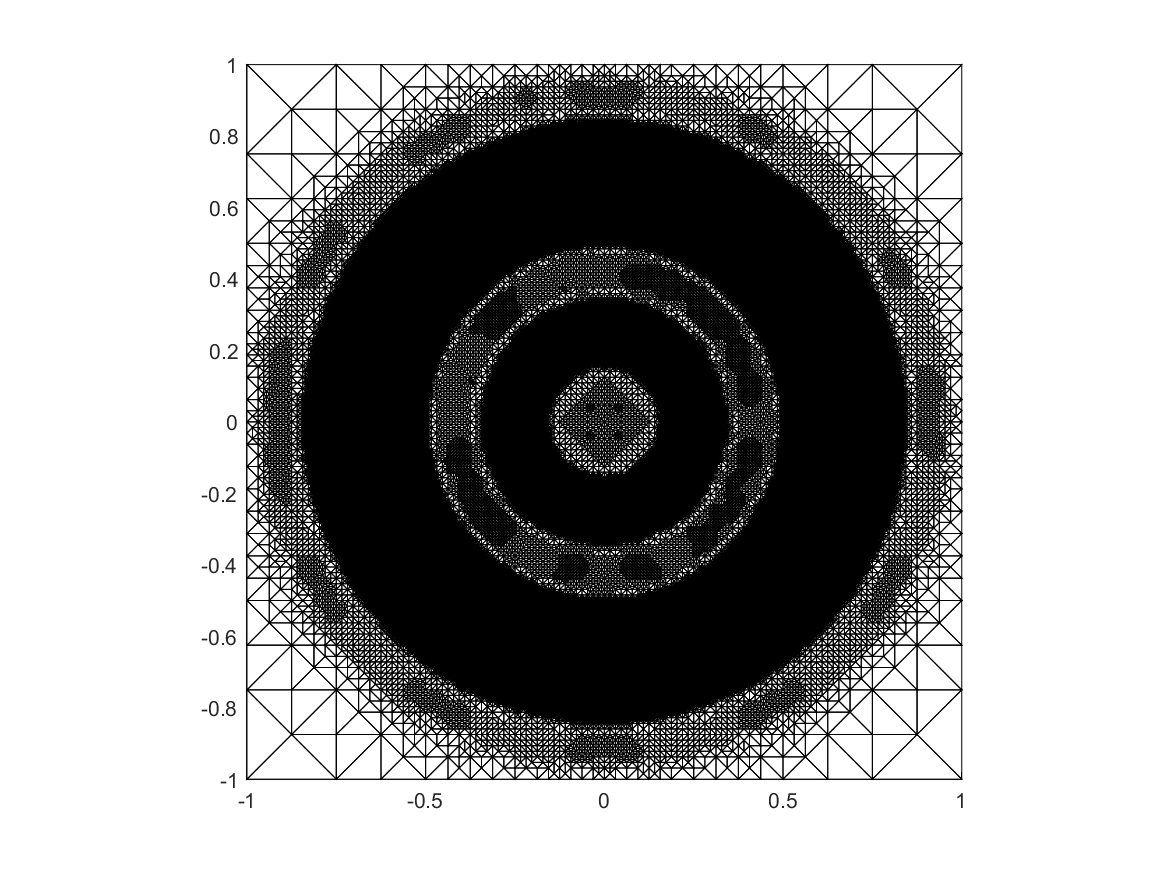
\includegraphics[trim = 100 30 80 20, clip, width=\linewidth]
      {pictures/chapExperiments/secExactSol/parGamma/5em1/lvl14/triangulation.png}
    \label{fig:gammaDot5Triang}
  \end{subfigure}
  \begin{subfigure}{.32\linewidth}
    \centering
    \caption{$\gamma=1$, $\text{nrDof}\approx 740\,000$}
    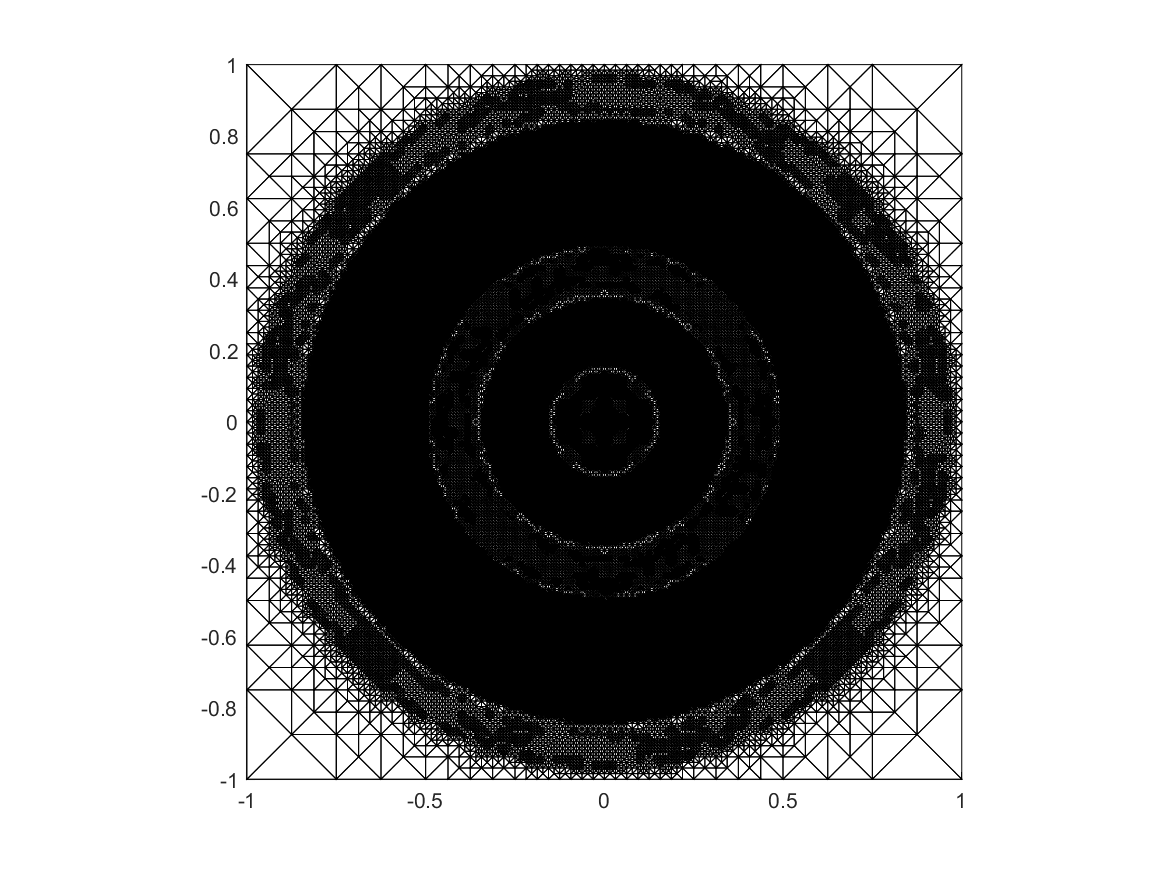
\includegraphics[trim = 100 30 80 20, clip, width=\linewidth]
      {pictures/chapExperiments/secExactSol/parGamma/1/lvl14/triangulation.png}
    \label{fig:gamma1Triang}
  \end{subfigure}
  \caption{Triangulierungen des jeweils letzten Levels 14 der Rechnungen mit
    verschiedenen Werten von $\gamma$ für das Eingangssignal $f_1$}
  \label{fig:gammaTriangs}
\end{figure}
In \Cref{fig:gammaTriangs} ist die Wirkung des Verfeinerungsindikators gut zu
erkennen. 
Die Kantensprünge sind dort am größten, wo die Lösung $u$, und damit die
meisten Iterate, nicht konstant sind.   
Dementsprechend wird mit kleinerem $\gamma$ stark dort verfeinert, wo die Lösung
$u$ aus \Cref{fig:f01Plots} nicht konstant ist.
Dies ist zu erkennen, obwohl die abgebildeten Triangulierungen für kleine
$\gamma$ deutlich mehr Freiheitsgrade haben als für $\gamma=1$.
Da wir im Experiment zu \Cref{fig:f01Convergence} bereits gesehen habe, dass
die Konvergenzraten bei adaptiver Netzverfeinerung nicht besser sind als bei
uniformer Netzverfeinerung, ist die ausbleibende Verbesserung der Ergebnisse
durch eine für $\gamma<1$ adaptivere Verfeinerung nicht unerwartet.
Insgesamt halten wir fest, dass die zu Beginn des Kapitels getroffene Wahl
von $\gamma=1$ weiterhin sinnvoll bleibt, da diese keinen Einfluss
auf die Fehlergraphen zu haben scheint, aber bessere Konvergenzraten
des Verfeinerungsindikators und seiner Anteile im Vergleich zu kleineren
Werten von $\gamma$ bewirkt.
Auch hier möchten wir anmerken, dass Ungleichung
\eqref{eq:expectedInequalities} für alle Wahlen von $\gamma$ erfüllt ist.

Zum Abschluss diese Abschnitts wollen wir die Experimente mit Eingangssignal
$f_1$ aus \Cref{fig:f01Convergence} noch mit $\alpha=10^4$ betrachten, das
heißt mit Eingangssignal $f_{10^4}$, und die Ergebnisse vergleichen.
\begin{figure}[p]
  \centering
  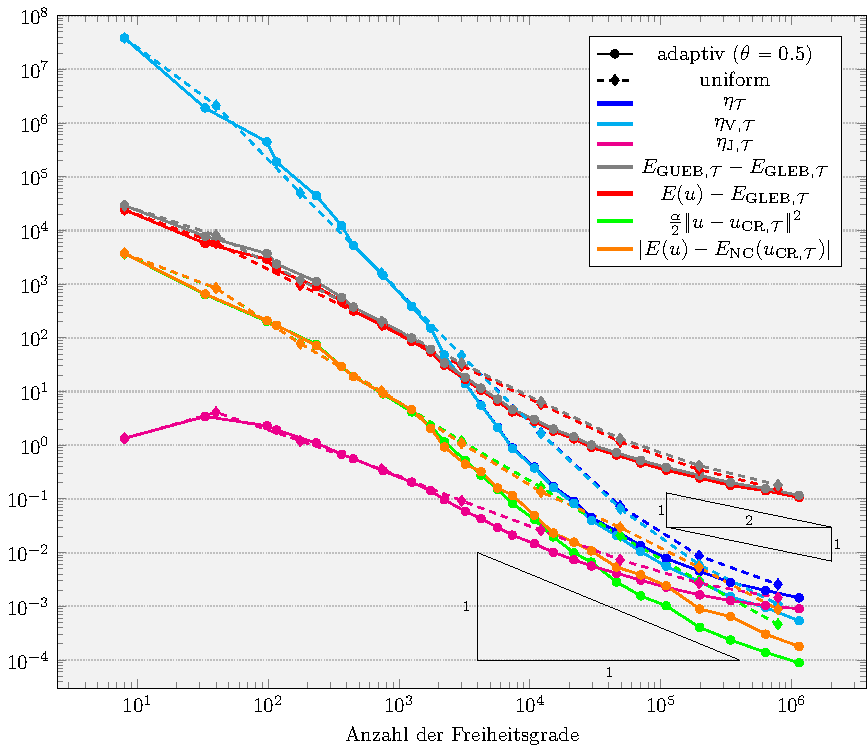
\includegraphics[width=.8\linewidth]
    {pictures/chapExperiments/secExactSol/f01LargeAlpha/conv.pdf}
  \caption{Ergebnisse der Rechnungen mit adaptiver und uniformer 
    Netzverfeinerung für das Eingangssignal $f_{10^4}$}
  \label{fig:f01LargeAlphaConvergence}
\end{figure}
Die Konvergenzraten in \Cref{fig:f01LargeAlphaConvergence} sind während eines
vorasymptotischen Bereichs, der bei etwa $10^5$ Freiheitsgraden endet, größer.
Danach sehen wir bei allen Graphen, außer dem für $|E(u)-\Enc(\ucrt)|$, die
anscheinend gleichen Raten, die wir schon in \Cref{fig:f01Convergence}
beobachtetet haben. 
Die Konvergenzrate von $|E(u)-\Enc(\ucrt)|$ scheint nun $1$ statt wie zuvor
1/2 zu sein.
Ansonsten gibt es nur zwei weitere nennenswerte Unterschiede.
Zum einen dominiert $\etaV$ hier lange den Verfeinerungsindikator, 
wobei ab etwa $10^6$ Freiheitsgraden die Dominanz von $\etaJ$ zu 
beginnen scheint, zum anderen erreichen alle Graphen, mit Ausnahme des
quadrierten exakten Fehlers und $\etaV$, geringere Werte nach $10^6$
Freiheitsgraden als für das Eingangssignal $f_1$.
Die Existenz des großen vorasymptotischen Bereichs wird möglicherweise dadurch
verursacht, dass für $\alpha=10^4$ alle Graphen, abgesehen von
$\etaJ$, zu Beginn des AFEM-Algorithmus deutlich größere Werte annehmen als für 
$\alpha =1$. 
Das Eingangssignal $f_{10^4}$ nimmt ebenfalls signifikant größere Werte an als
$f_1$.
Die Iterationen auf den ersten Leveln der AFEM-Routine erreichen dann jeweils
starke Reduktionen der betrachteten Terme und bedingen somit den
vorasymptotischen Bereich.
Die Ungleichung \eqref{eq:expectedInequalities} ist auch hier stets gültig,


\section{Graufarbenbilder als Eingangssignale}
\label{sec:grayscalePicturesAsInputSignal}

In diesem Abschnitt wollen wir Ergebnisse von Experimenten untersuchen, bei
denen als Eingangssignal ein
Graufarbenbild nach \Cref{rem:grayscalePictureInputSignal} gegeben ist.
Für diese Rechnungen sind entsprechend weder exakte Lösung noch die schwache
Ableitung des Eingangssignals bekannt.
Zunächst betrachten wir das Eingangssignal \texttt{cameraman} aus
\Cref{fig:cameraman}. 
\begin{figure}[p]
  \centering
  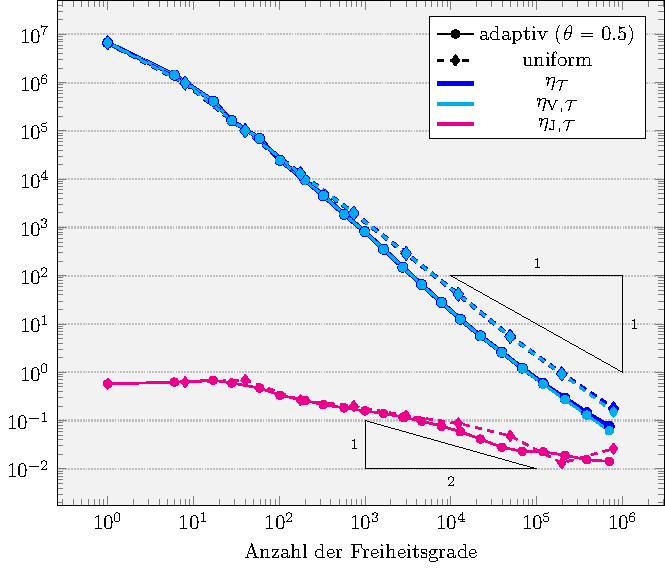
\includegraphics[width=.8\linewidth]
    {pictures/chapExperiments/secGrayscale/cam/conv.pdf}
  \caption{Ergebnisse der Rechnungen mit adaptiver und uniformer 
    Netzverfeinerung für das Eingangssignal \texttt{cameraman}}
  \label{fig:camConvergence}
\end{figure}
In \Cref{fig:camConvergence} sehen wir für den Verfeinerungsindikator $\etaT$
und dessen Anteil $\etaV$ die Konvergenzrate $1$.
Für den Anteil $\etaJ$ von $\etaT$ ist ungefähr die Rate $1/2$ zu erkennen, 
wobei $\etaJ$ bei uniformer Netzverfeinerung für das letzte Level einen
etwas größeren Wert annimmt als für das vorletzte.
Ansonsten ist bei den Konvergenzraten kein Unterschied zwischen uniformer und
adaptiver Netzverfeinerung festzustellen.
Die Raten von $\etaV$ und $\etaJ$ stimmen mit den Raten überein, die schon beim
Experiment mit Eingangssignal $f_1$ in \Cref{fig:f01Convergence} beobachtet
wurden, wobei hier der Verfeinerungsindikator von $\etaV$ dominiert wird und
nicht, wie beim Experiment mit Eingangssignal $f_1$, von $\etaJ$.
Dementsprechend konvergiert hier $\etaT$ auch nicht mit der Rate 1/2, sondern
mit der Rate $1$.
Weiterhin nimmt $\etaV$, und somit auch $\etaT$, im Vergleich zur Rechnung mit
Eingangssignal $f_1$ zu Beginn der AFEM-Routine deutlich höhere Werte an.
Diese sind vergleichbar mit den beim Experiment mit Eingangssignal $f_{10^4}$
in \Cref{fig:f01LargeAlphaConvergence}, bei dem ebenfalls $\alpha=10^4$ gewählt
war, beobachteten Werten. 
Bei einer Rechnung mit einem Eingangssignal $f$, bei dem $\alpha$ groß gewählt
ist im Vergleich zu einem anderen Experiment, scheinen also auf den ersten
Leveln der AFEM-Routine höhere Werte für $\etaV$ aufzutreten als in einem
Experiment mit einer kleineren Wahl von $\alpha$.
\begin{figure}[p]
  \centering
  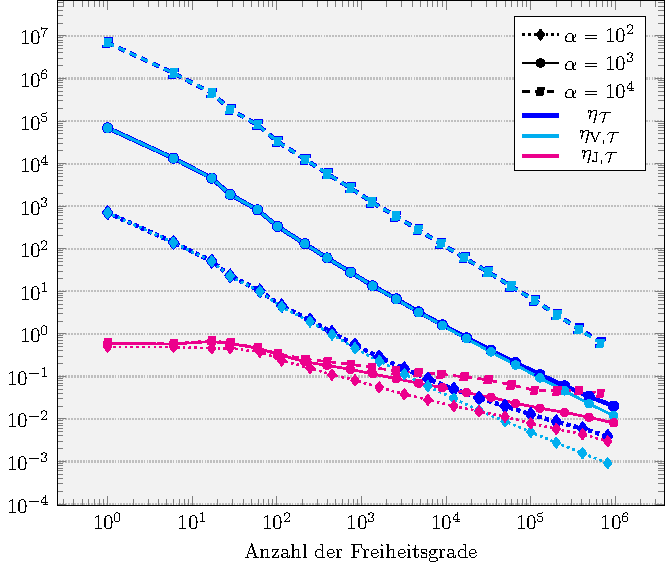
\includegraphics[width=.8\linewidth]
    {pictures/chapExperiments/secGrayscale/denoise/conv.pdf}
  \caption{Ergebnisse der Rechnungen zu \Cref{fig:exampleDenoising} für drei
    verschiedene Werte von $\alpha$}
  \label{fig:denoiseConvergence}
\end{figure}
Dies wird bekräftigt in \Cref{fig:denoiseConvergence}, in der wir
die Konvergenzgraphen zu \Cref{fig:exampleDenoising} vergleichen für
$\alpha\in\{10^2,10^3,10^4\}$ und ebendieses Verhalten beobachten.
Ein Grund dafür könnte sein, dass, wenn $\alpha$ groß gewählt wird, die Terme
$\Vert f-\alpha \ucrt\Vert^2_{L^2(T)}$ im Anteil $\etaV$ des
Verfeinerungsindikators aus \Cref{def:refinementIndicator} für viele Dreiecke
$T\in\Tcal$ ebenfalls größere Werte annehmen als für ein Experiment mit einer
kleineren Wahl für $\alpha$.
Zum Abschluss diese Abschnitts möchten wir anhand des Beispiels mit
Eingangssignal \texttt{cameraman} die Wirkung des Verfeinerungsindikators
veranschaulichen.
\begin{figure}[p]
  \centering
  \begin{subfigure}[b]{.48\linewidth}
    \centering
    \caption{Triangulierung Level 17}
    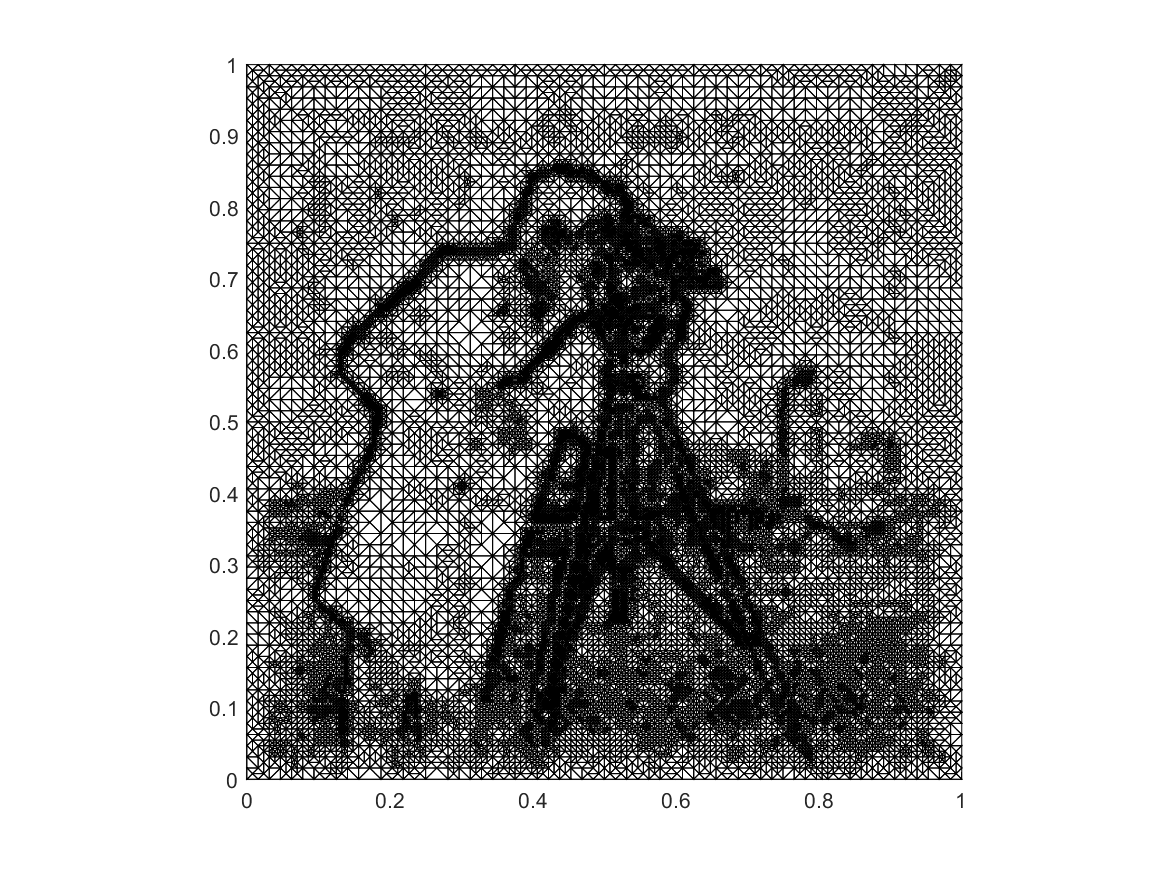
\includegraphics[trim = 100 30 80 20, clip, width=\linewidth]
      {pictures/chapExperiments/secGrayscale/cam/adaptive/lvl17/triangulation.png}
    \label{fig:camLvl17Triang}
  \end{subfigure}
  \quad
  \begin{subfigure}[b]{.48\linewidth}
    \centering
    \caption{Lösung Level 17}
    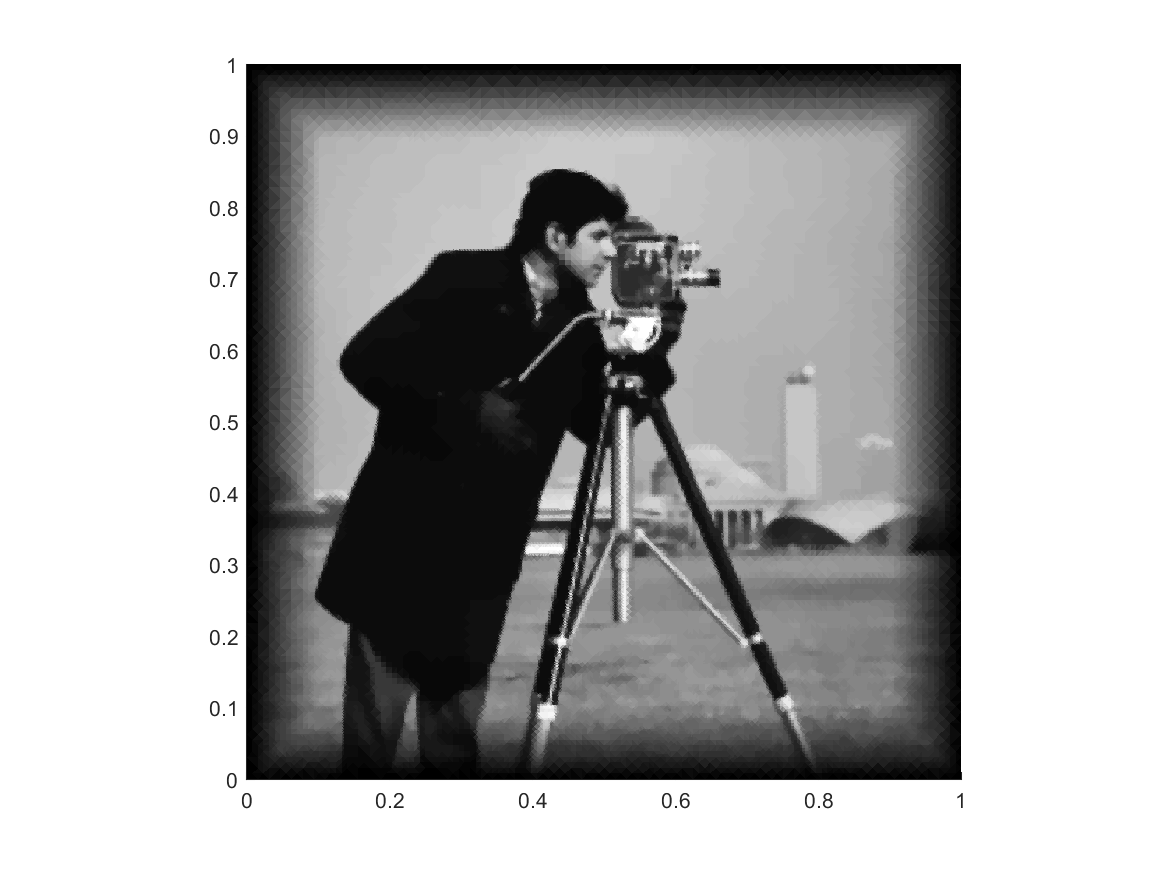
\includegraphics[trim = 100 30 80 20, clip, width=\linewidth]
      {pictures/chapExperiments/secGrayscale/cam/adaptive/lvl17/solutionGrayscale.png}
    \label{fig:camLvl17Sol}
  \end{subfigure}

  \begin{subfigure}[b]{.48\linewidth}
    \centering
    \caption{Triangulierung Level 21}
    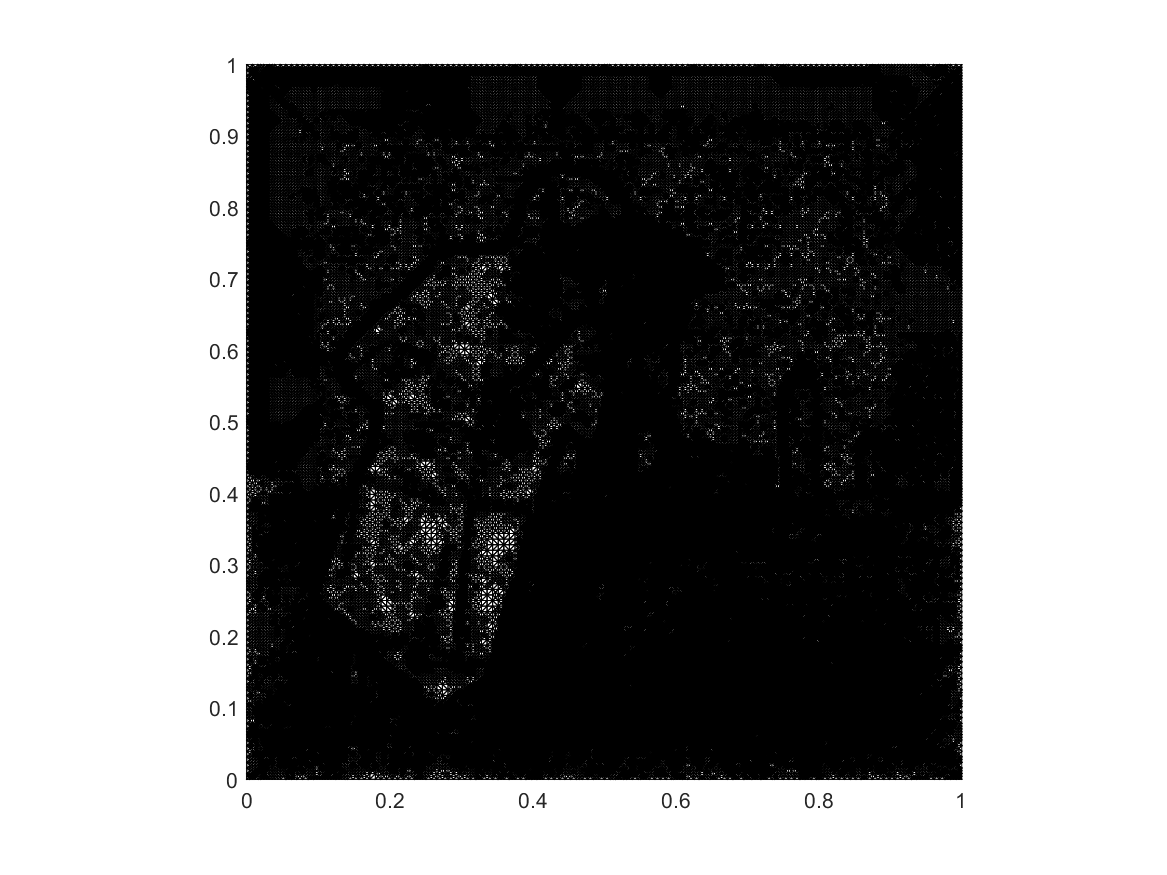
\includegraphics[trim = 100 30 80 20, clip, width=\linewidth]
      {pictures/chapExperiments/secGrayscale/cam/adaptive/lvl21/triangulation.png}
    \label{fig:camLvl21Triang}
  \end{subfigure}
  \quad
  \begin{subfigure}[b]{.48\linewidth}
    \centering
    \caption{Lösung Level 21}
    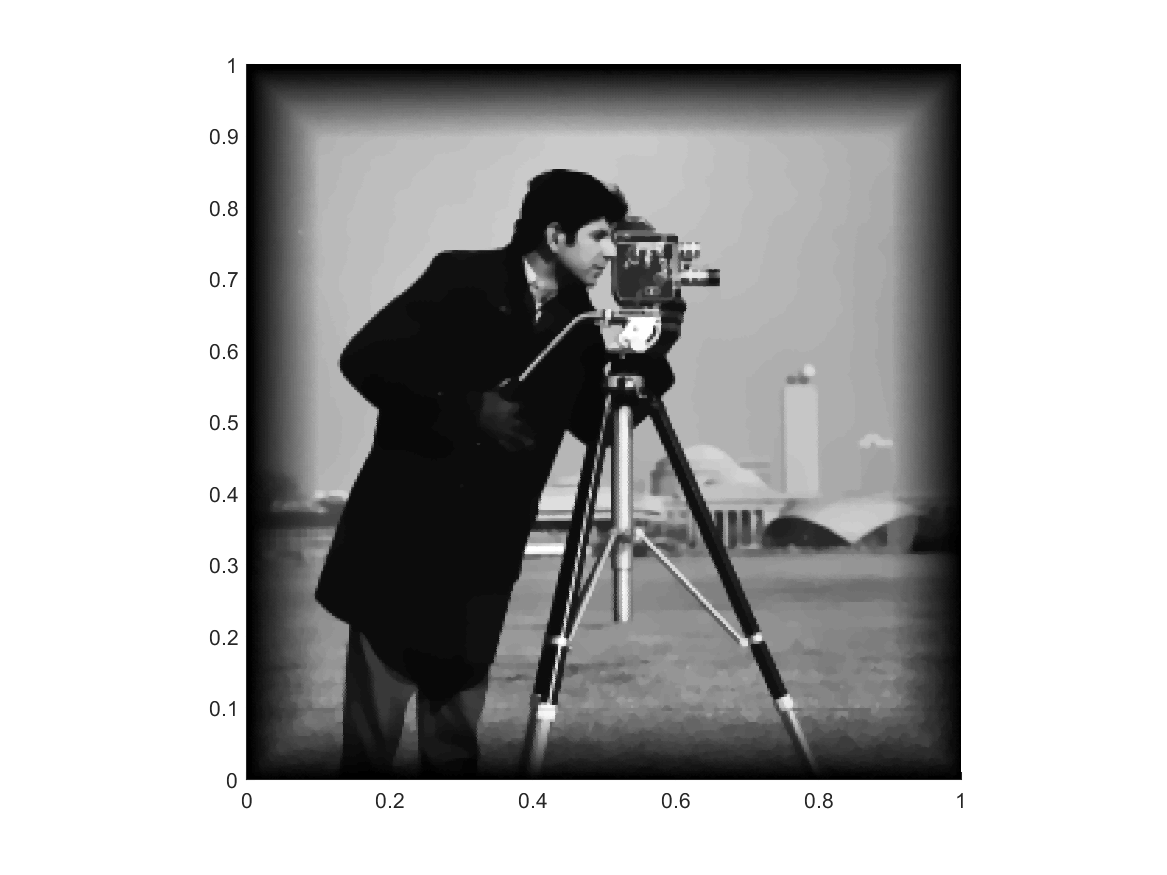
\includegraphics[trim = 100 30 80 20, clip, width=\linewidth]
      {pictures/chapExperiments/secGrayscale/cam/adaptive/lvl21/solutionGrayscale.png}
    \label{fig:camLvl21Sol}
  \end{subfigure}
  \caption{Triangulierung und diskrete Lösung, als Graufarbenplot aus der
    Draufsicht, nach der Rechnung mit Eingangssignal \texttt{cameraman} für
    Level 17 des AFEM-Algorithmus nach etwa 70\,000 Freiheitsgraden und für
    Level 21 nach etwa 700\,000 Freiheitsgraden}
  \label{fig:camTriang}
\end{figure}
Wir sehen in \Cref{fig:camLvl17Triang} gut, dass dieser eine Verfeinerung zu
den Unstetigkeiten bewirkt, insbesondere zu denen entlang deutlicher
Farbkontraste.
Außerdem ist zu erkennen, dass der hinzufügte graduelle Übergang zu schwarzem
Rand für das Eingangssignal den gewünschten Effekt hat, eine starke
Verfeinerung zum Rand, die aufgrund der angenommenen Nullranddaten passieren
würde, zu verhindern.
Somit wird tatsächlich dort stark verfeinert, wo mehr Informationen benötigt
werden, was am Rand nicht der Fall wäre.
Auch in \Cref{fig:camLvl21Triang} kann man, trotz der hohen Anzahl an
Freiheitsgaden, noch erkennen, wo es im Bild kaum Farbkontraste gibt und eine
Verfeinerung deshalb nicht unbedingt nötig ist.
Die diskrete Lösung ähnelt dem Eingangssignal, was aufgrund der großen Wahl für
$\alpha$ nach der Interpretation des ROF-Modellproblems aus
\Cref{chap:introduction} zu erwarten war.


\section{Stetige Approximation eines unstetigen Eingangssignals}

Diese Experimente nutzen als die initiale Triangulierung aus
\Cref{fig:triangBigSquare}.
Da wir nun gesehen haben, dass die Raten für $\etaV$ und $\etaJ$ übereinstimmen
mit den beobachteten Raten im vorherigen
\Cref{sec:experimentsWithExactSolution}, interessiert uns ob noch weitere
Raten vergleichbar sind. 
Allerdings haben wir beim Eingangssignal \texttt{cameraman} das Problem,
weder Gradienten noch die exakte Lösung zu kennen und so entsprechend keine
der anderen Graphen plotten zu können.
Deshalb betrachten wir ein weiteres Beispiel mit Unstetigkeitsmenge und 
eine kontinuierliche Approximation dieser, für die wir nach
\Cref{sec:constructionInputSignal} eine exakte Lösung kennen.
Als unstetige Funktion, die als Graufarbenbild interpretiert einem 
weißen Kreis mit Radius $1/2$ entspricht, betrachten wir die Funktion
\begin{align*}
  f_\textrm{DC}(r)\coloneqq 
  \begin{cases}
    10^4, 
    & \text{falls } r\in \left[0,\frac{1}{2}\right]\!,\\
    0, 
    & \text{falls } r\in \left(\frac{1}{2},\infty\right)\!.
  \end{cases}
\end{align*}
Betrachten wir nun die Funktion
\begin{align*}
  u_\textrm{C}(r)\coloneqq 
  \begin{cases}
    1, 
    & \text{falls } r\in \left[0,\frac{1-\beta}{2}\right]\!,\\
    -\frac{1}{\beta}r + \frac{1+\beta}{2\beta}, 
    & \text{falls } r\in \left(\frac{1-\beta}{2}, \frac{1+\beta}{2}\right]\!,\\
    0,
    & \text{falls } r\in \left(\frac{1+\beta}{2},\infty\right)\!,
  \end{cases}
\end{align*}
erhalten wir mit der Wahl
\begin{align*}
  \sgn(\partial_r u_\textrm{C}(r)) 
  &\coloneqq 
  \begin{cases}
    \frac{4}{1-\beta}r\left(\frac{1}{1-\beta}r -1\right)\!, 
    & \text{falls } r\in \left[0,\frac{1-\beta}{2}\right]\!,\\
    -1,
    & \text{falls } r\in \left(\frac{1-\beta}{2}, \frac{1+\beta}{2}\right]\!,\\
    \frac{4}{(\beta-1)^3}
    \left( 4r^3-3(\beta+3)r^2 +6(\beta+1)r-3\beta-1\right)\!, 
    & \text{falls } r\in \left(\frac{1+\beta}{2},\infty\right)\!,
  \end{cases}
\end{align*}
die rechte Seite
\begin{align*}
  f_\textrm{C}(r)\coloneqq 
  \begin{cases}
    \alpha - \frac{4}{1-\beta}\left(\frac{3}{1-\beta}r - 2\right)\!, 
    & \text{falls } r\in \left[0,\frac{1-\beta}{2}\right]\!,\\
    -\frac{\alpha}{\beta}\left( r-\frac{1+\beta}{2} \right) +\frac{1}{r}, 
    & \text{falls } r\in \left(\frac{1-\beta}{2}, \frac{1+\beta}{2}\right]\!,\\
    \frac{-4}{(\beta-1)^3}
    \left( 16r^2 -9(\beta+3)r + 12(\beta+1) - \frac{3\beta+1}{r}\right)\!, 
    & \text{falls } r\in \left(\frac{1+\beta}{2},\infty\right)\!.
  \end{cases}
\end{align*}
Die entsprechenden Ableitungen sind
\begin{align*}
  \partial_r f_\textrm{C}(r) &= 
  \begin{cases}
    -\frac{12}{(1-\beta)^2},
    & \text{falls } r\in \left[0,\frac{1-\beta}{2}\right]\!,\\
    -\frac{\alpha}{\beta}-\frac{1}{r^2},
    & \text{falls } r\in \left(\frac{1-\beta}{2}, \frac{1+\beta}{2}\right]\!,\\
    -\frac{4}{(1-\beta)^3}\left( 32r-9(\beta+3)+\frac{3\beta+1}{r^2} \right)\!,
    & \text{falls } r\in \left(\frac{1+\beta}{2},\infty\right)\!,
  \end{cases}
\end{align*}
und
\begin{align*}
  \partial_r u_\textrm{C}(r) &= 
  \begin{cases}
    0,
    & \text{falls } r\in \left[0,\frac{1-\beta}{2}\right]\!,\\
    -\frac{1}{\beta},
    & \text{falls } r\in \left(\frac{1-\beta}{2}, \frac{1+\beta}{2}\right]\!,\\
    0,
    & \text{falls } r\in \left(\frac{1+\beta}{2},\infty\right)\!,
  \end{cases}
\end{align*}
womit wir die Energie
$E(u)\approx -3\,924.37413$ für das Experiment mit $\alpha=10^4$ und $\beta =
10^{-3}$ erhalten.
\begin{figure}[p]
  \centering
  \begin{subfigure}[b]{.48\linewidth}
    \centering
    \caption{Insi circle stetig entlang der Achsen}
    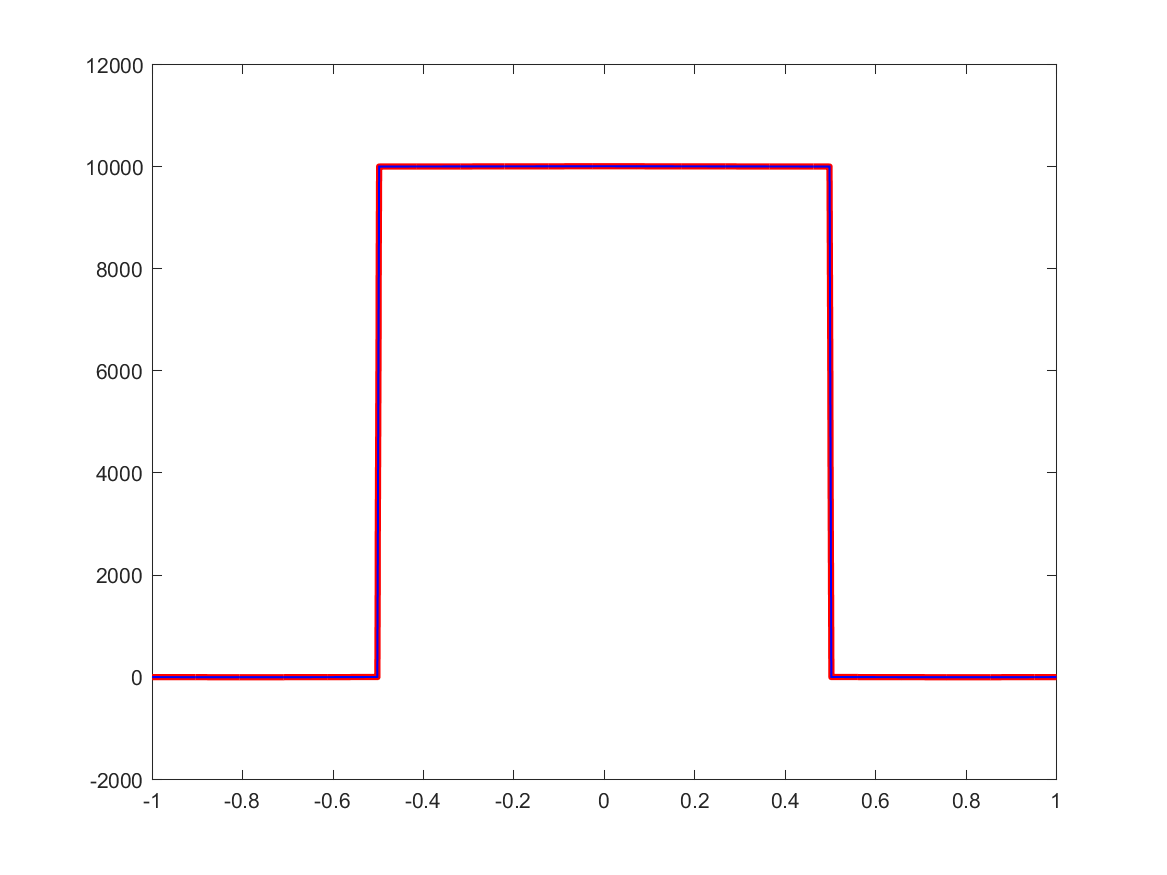
\includegraphics[trim = 40 30 50 20, clip, width=\linewidth]
      {pictures/chapExperiments/secGrayscale/circ/cont/inSiAxis.png}
    \label{fig:circContInSiAxis}
  \end{subfigure}
  \quad
  \begin{subfigure}[b]{.48\linewidth}
    \centering
    \caption{Exakte Lsg circle stetig entlang der Achsen}
    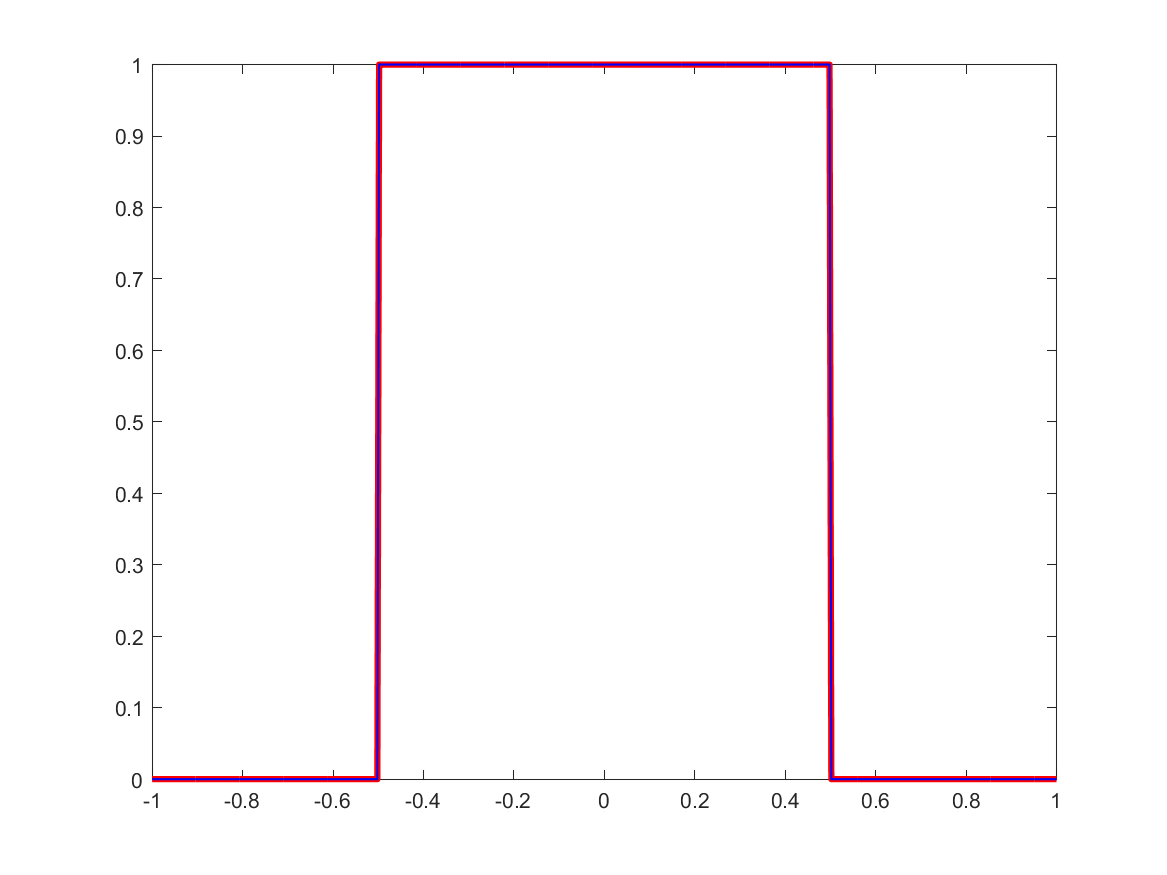
\includegraphics[trim = 40 30 50 20, clip, width=\linewidth]
      {pictures/chapExperiments/secGrayscale/circ/cont/exactSolutionAxis.png}
    \label{fig:circContExactSolAxis}
  \end{subfigure}
  \caption{InSi und exakte Lösung circle stetig entlang der Achsen.}
  \label{fig:circContPlotsAxis}
\end{figure}
Augenscheinlich ist $f_\textrm{C}$ für diese Wahl von $\alpha$ und $\beta$ eine
stetige Approximation von $f_\textrm{DC}$, wie in \Cref{fig:circContPlotsAxis}
zu sehen ist.
Außerdem sehen wir dort auch wieder für dieses große $\alpha$ das erwarte
Verhalten, dass das Eingangssignal ungefähr gleich dem Produkt aus $\alpha$ und
der exakten Lösung zu sein scheint, wie nach \Cref{chap:introduction} erwartet.
\begin{figure}[p]
  \centering
  \begin{subfigure}[b]{.48\linewidth}
    \centering
    \caption{adaptive Konvergenz vergleich stetig und unstetig}
    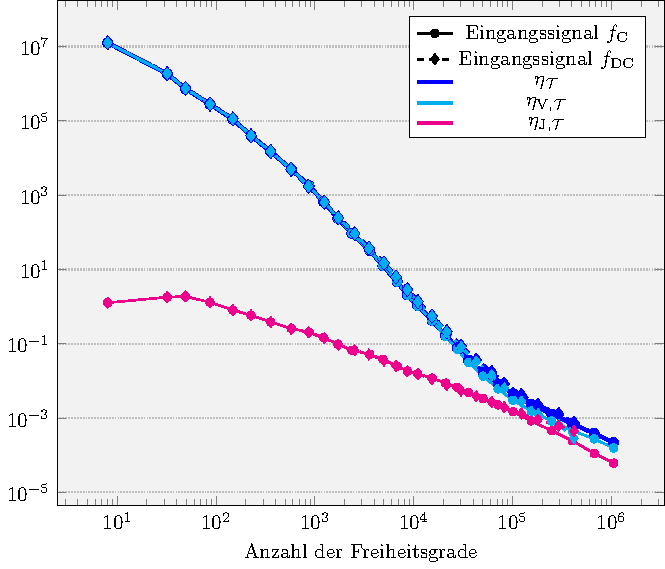
\includegraphics[width=\linewidth]
      {pictures/chapExperiments/secGrayscale/circ/convAdap.pdf}
    \label{fig:circConvAdaptive}
  \end{subfigure}
  \quad
  \begin{subfigure}[b]{.48\linewidth}
    \centering
    \caption{uniforme Konvergenz vergleich stetig und unstetig}
    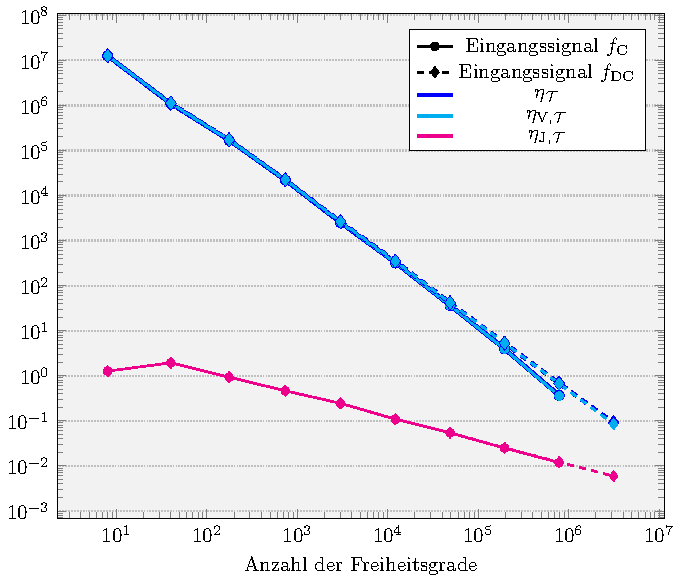
\includegraphics[width=\linewidth]
      {pictures/chapExperiments/secGrayscale/circ/convUnif.pdf}
    \label{fig:circConvUniform}
  \end{subfigure}
  \caption{adptive und uniformer Vergleich für circle stetig und unstetig}
  \label{fig:circConvComparison}
\end{figure}
Zunächst sehen wir in \Cref{fig:circConvComparison} sowohl für adaptive
als auch uniforme Netzverfeierung, dass es für die beiden Eingangssignal 
bis $10^6$ Freiheitsgrade keine deutlichen Unterschiede im Verlauf
des Verfeinerungsindikators und seiner Anteile gibt. 
\begin{figure}[p]
  \centering
  \begin{subfigure}[b]{.48\linewidth}
    \centering
    \caption{Eingangssignal $f_\textup{C}$, Level 17}
    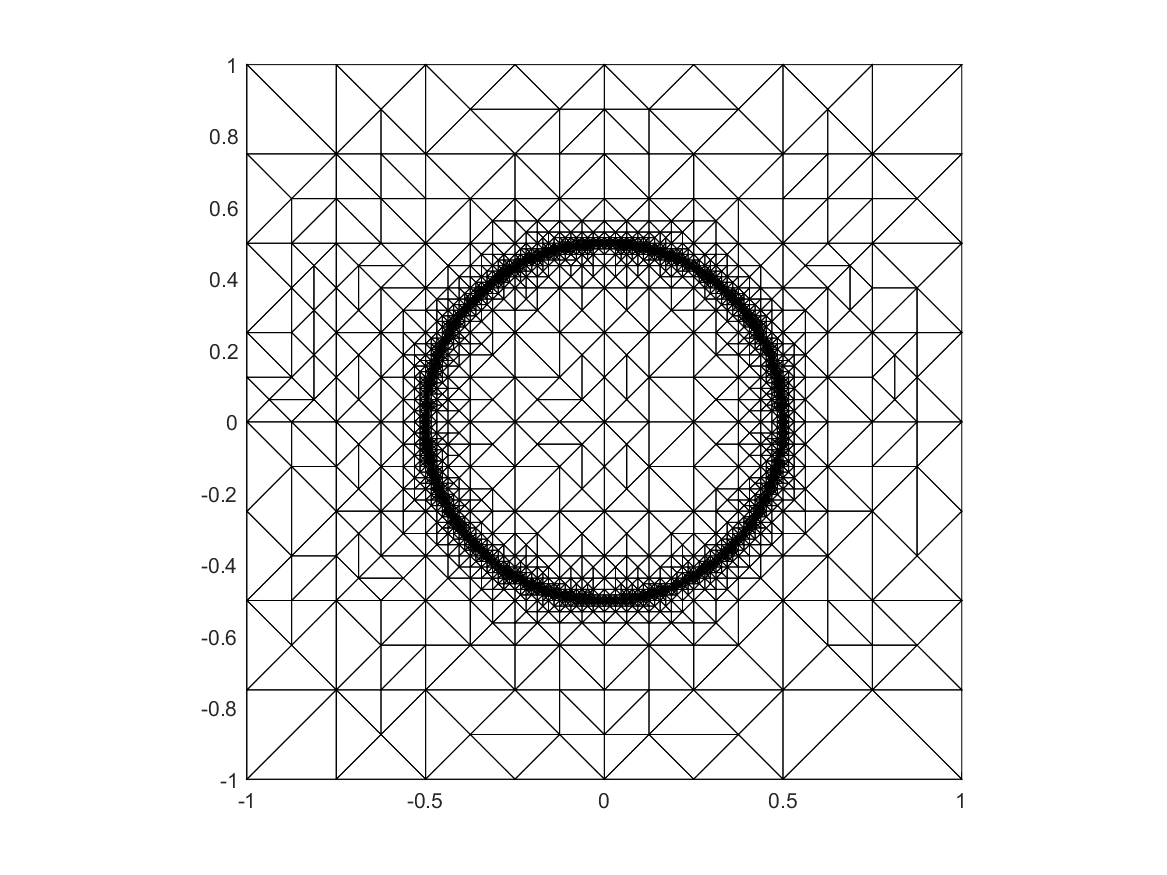
\includegraphics[trim = 100 30 80 20, clip, width=\linewidth]
      {pictures/chapExperiments/secGrayscale/circ/cont/adaptive/lvl17/triangulation.png}
    \label{fig:circContLvl17Triang}
  \end{subfigure}
  \quad
  \begin{subfigure}[b]{.48\linewidth}
    \centering
    \caption{Eingangssignal $f_\textup{DC}$, Level 17}
    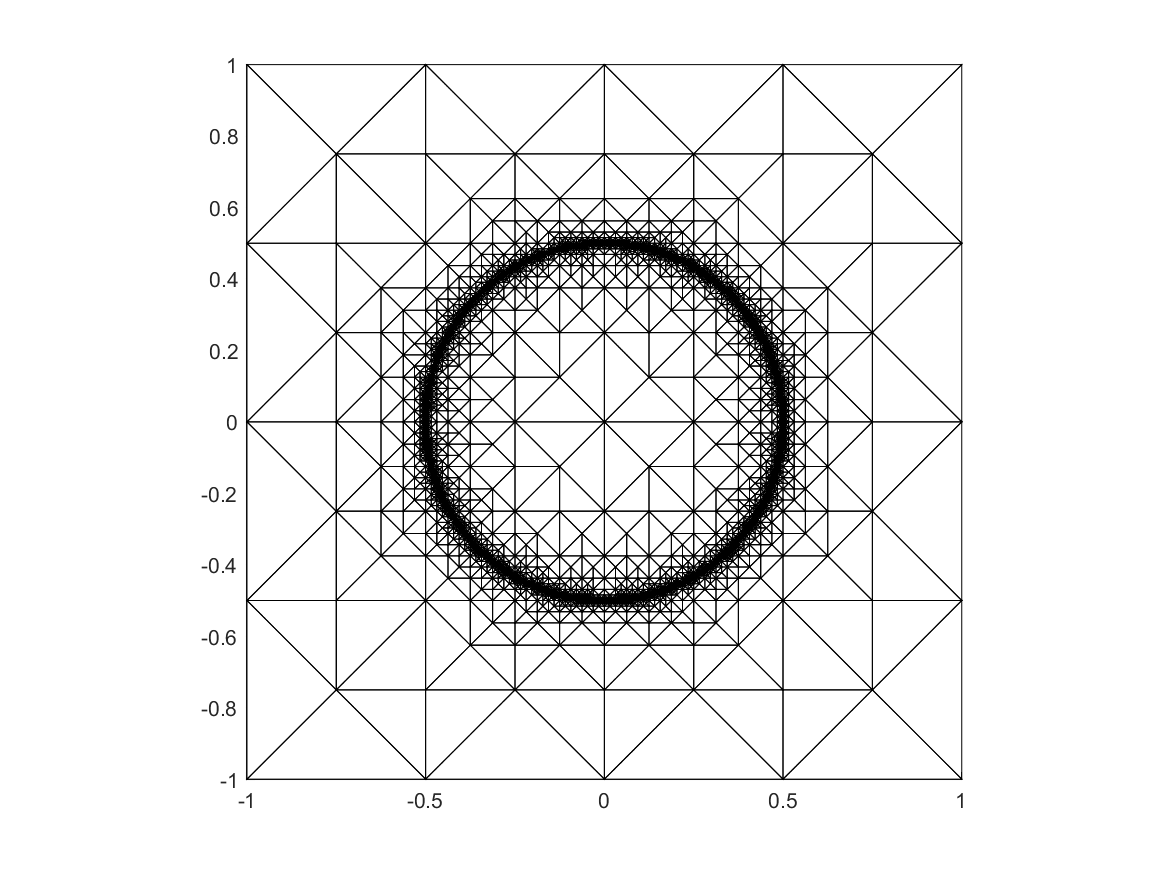
\includegraphics[trim = 100 30 80 20, clip, width=\linewidth]
      {pictures/chapExperiments/secGrayscale/circ/disc/adaptive/lvl17/triangulation.png}
    \label{fig:circDiscLvl17Triang}
  \end{subfigure}
%
%  \begin{subfigure}[b]{.48\linewidth}
%    \centering
%    \caption{Eingangssignal $f_\textup{C}$, Level 26}
%    \includegraphics[trim = 100 30 80 20, clip, width=\linewidth]
%      {pictures/chapExperiments/secGrayscale/circ/cont/adaptive/lvl26/triangulation.png}
%    \label{fig:circContFinalTriang}
%  \end{subfigure}
%  \quad
%  \begin{subfigure}[b]{.48\linewidth}
%    \centering
%    \caption{Eingangssignal $f_\textup{DC}$, Level 26}
%    \includegraphics[trim = 100 30 80 20, clip, width=\linewidth]
%      {pictures/chapExperiments/secGrayscale/circ/disc/adaptive/lvl26/triangulation.png}
%    \label{fig:circDiscFinalTriang}
%  \end{subfigure}
  \caption{Triangulierungen für die Eingangssignale $f_\textup{C}$ und
  $f_\textup{DC}$ für Level 17 und Level 26 des jeweiligen adaptiven
  Algorithmus mit etwa 15\,000 Freiheitsgraden für Level 26 und etwa 400\,000
  Freiheitsgraden für Level 26}
  \label{fig:circleTriang}
\end{figure}
\begin{figure}[p]
  \centering
  \begin{subfigure}[b]{.48\linewidth}
    \centering
    \caption{Lösung circ stetig}
    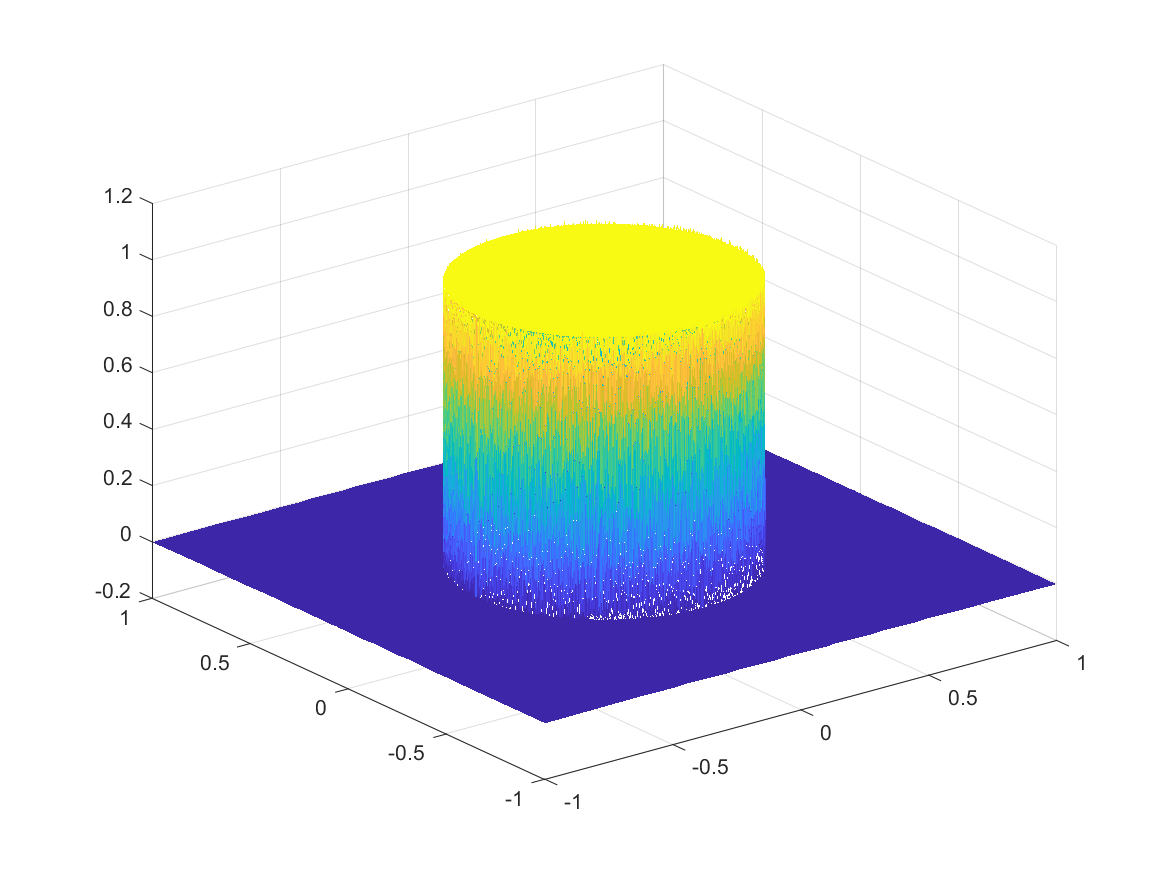
\includegraphics[trim = 40 30 30 30, clip, width=\linewidth]
      {pictures/chapExperiments/secGrayscale/circ/cont/adaptive/lvl28/solution.png}
    \label{fig:circContSol}
  \end{subfigure}
  \quad
  \begin{subfigure}[b]{.48\linewidth}
    \centering
    \caption{Lösuns stetig final entlang der Achsen}
    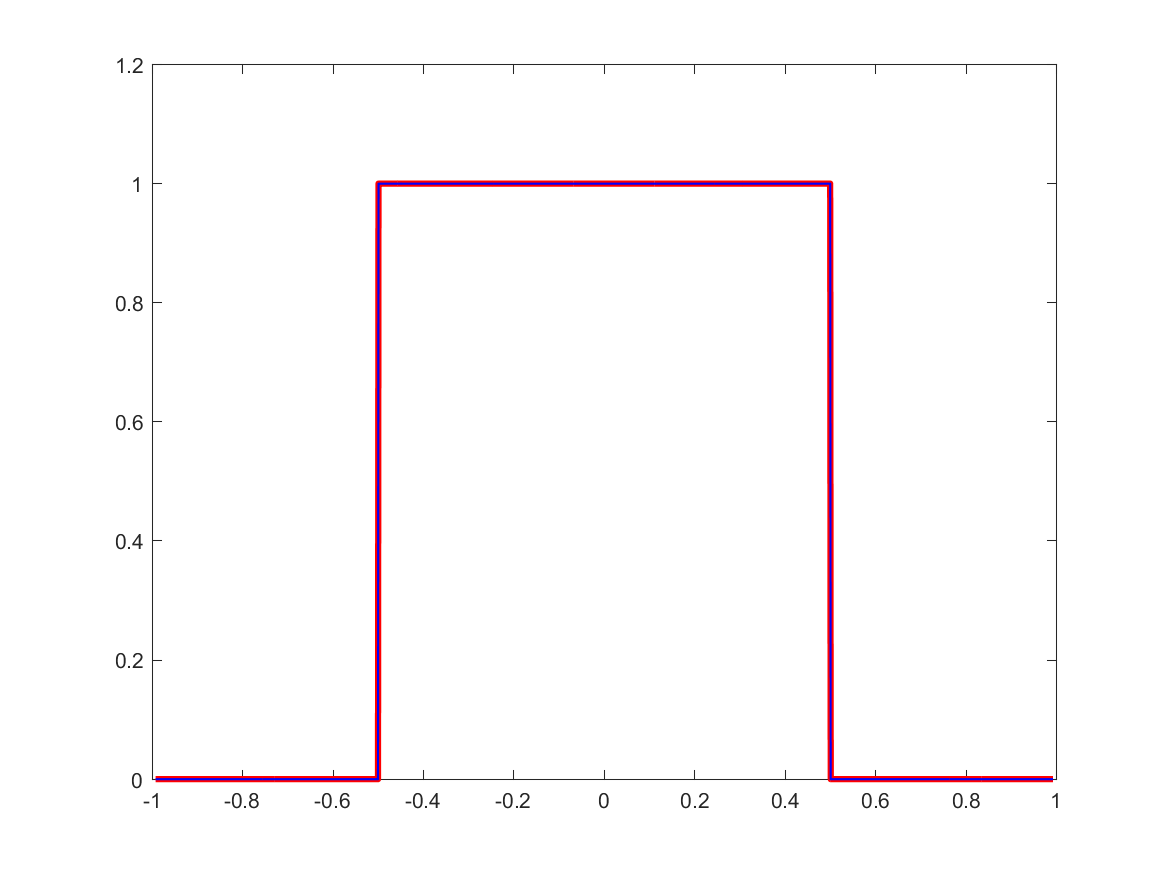
\includegraphics[trim = 50 30 50 20, clip, width=\linewidth]
      {pictures/chapExperiments/secGrayscale/circ/cont/adaptive/lvl28/solutionAxis.png}
    \label{fig:circContSolAxis}
  \end{subfigure}

  \begin{subfigure}[b]{.48\linewidth}
    \centering
    \caption{Lösung circ unstetig}
    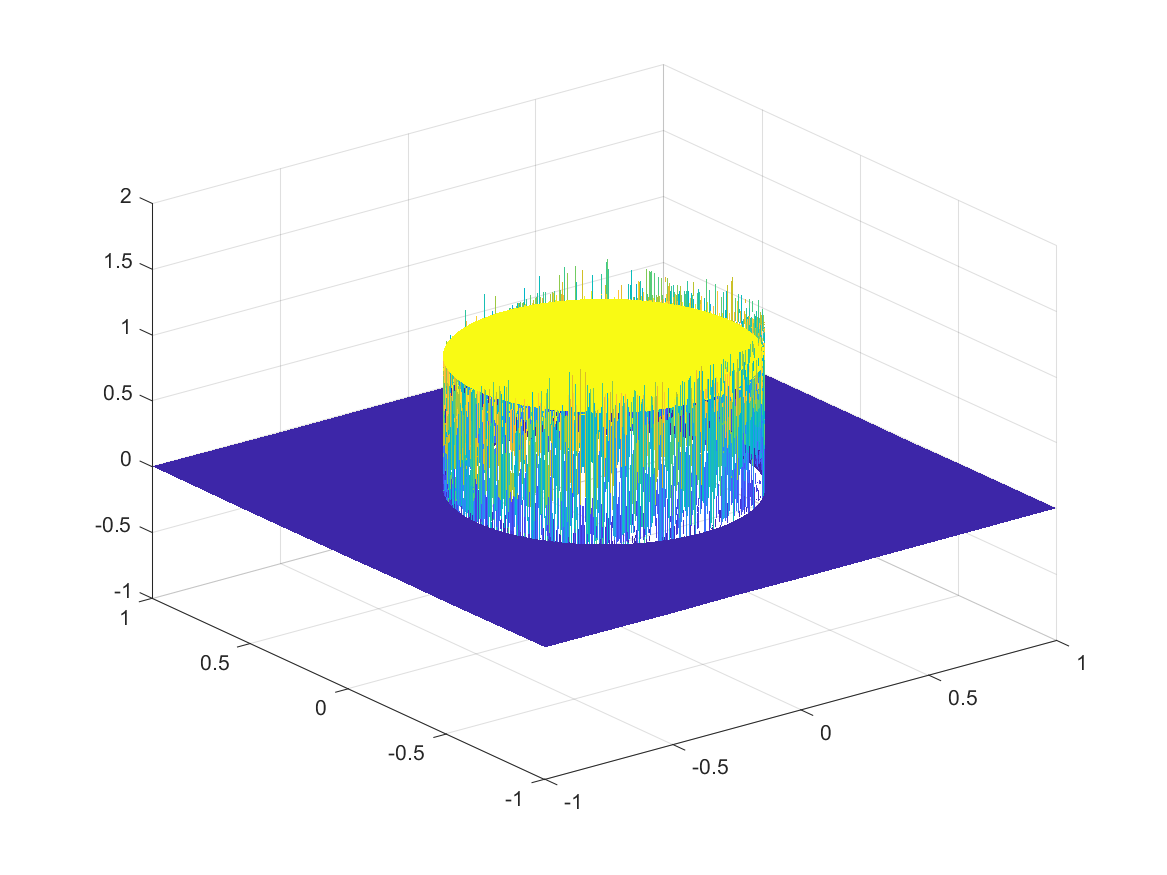
\includegraphics[trim = 40 30 30 30, clip, width=\linewidth]
      {pictures/chapExperiments/secGrayscale/circ/disc/adaptive/lvl26/solution.png}
    \label{fig:circDiscSol}
  \end{subfigure}
  \quad
  \begin{subfigure}[b]{.48\linewidth}
    \centering
    \caption{Lösuns unstetig final entlang der Achsen}
    \includegraphics[trim = 50 30 50 20, clip, width=\linewidth]
      {pictures/chapExperiments/secGrayscale/circ/disc/adaptive/lvl26/solutionAxis.png}
    \label{fig:circDiscSolAxis}
  \end{subfigure}
  \caption{Lösung für Eingangssignal circle stetig und unstetig, wobei die
  augenscheinliche Stetigkeit der Lösung für Eingangssignal $f_\textup{DC}$
  bei $1/2$ nur durch den Plot bedingt ist.}
  \label{fig:circleSol}
\end{figure}
% TODO Freiheitsgrade ergänzen bei den Triangulierungen sobald fertig,
% außerdem auf vergleichbare Anzahl von Freiheitsgraden achten
In \Cref{fig:circleTriang} (TODO update und Freiheitsgrade ergänzen) ist
weiterhin zu sehen, dass auch der
Verfeinerungsindikator beim adaptiven Algorithmus eine vergleichbare und
erwarterte Verfeinerung zur Unstetigkeitsmenge vollzieht bei
Level 17 und sich die Verfeinerungen erst bei höheren Freiheitsgraden 
unterscheiden. 
Außerdem ähneln die in \Cref{fig:circleSol} dargestellten Lösungen der
adaptiven Algorithmen beide der exakten Lösung für das Eingangssignal
$f_\textup{C}$ aus \Cref{fig:circContExactSolAxis}.
Insgesamt scheinen die Ergebnisse beider Experiment tatsächlich vergleichbar
zu sein, weshalb wir nun das Experiment mit Eingangssignal $f_\textup{C}$
mit $\alpha=10^4$ und $\beta=10^{-3}$ weiter untersuchen möchten.
\begin{figure}[p]
  \centering
  \includegraphics[width=.8\linewidth]
    {pictures/chapExperiments/secGrayscale/circ/convCont.pdf}
  \caption{Ergebnisse für Eingangssignal circle stetig.}
  \label{fig:circContConvergence}
\end{figure}
In \Cref{fig:circContConvergence} ist zu sehen, dass wir hier ein Experiment
gefunden haben, bei der der adaptive Algorithmus bessere Raten als
der uniforme Algorithmus erzielt für den Fehler, die exakte Energiedifferenz
und $\etaJ$, jeweils mit Rate $1/2$ statt $1$.
Der Verfeinerungsindikator und $\etaV$ und die von $\Egleb$ abhängigen Graphen
scheinen zwar die gleichen Raten zu haben, allerdings erzielt der adaptive
Algorithmus deutlich geringere Werte.
Dies wird bei diesem Beispiel daran liegen, dass es klar nur sinnvoll sein
kann, bei der Unstetigkeit zu verfeinern, welche von der Triangulierung
natürlich nicht perfekt aufgelöst werden kann.
Diese Aussagen gelten demenstsprechend womöglich auch für $f_\textup{DC}$.
Dies zeigt, dass für Eingangssignale, bei denen
die Verfeinerung stark lokal sinnvoll ist, der adaptive Algorithmus 
ein besseres Konvergenzverhalten hat als der uniforme.
\begin{figure}[p]
  \centering
  \begin{subfigure}{.32\linewidth}
    \centering
    \caption{$f_\textup{C}$}
    \includegraphics[width=\linewidth]
      {pictures/chapExperiments/secGrayscale/circ/misc.pdf}
    \label{fig:miscCircle}
  \end{subfigure}
  \begin{subfigure}{.32\linewidth}
    \centering
    \caption{$f_1$}
    \includegraphics[width=\linewidth]
      {pictures/chapExperiments/secExactSol/f01/misc.pdf}
    \label{fig:miscF01}
  \end{subfigure}
  \begin{subfigure}{.32\linewidth}
    \centering
    \caption{\texttt{cameraman}}
    \includegraphics[width=\linewidth]
      {pictures/chapExperiments/secGrayscale/cam/misc.pdf}
    \label{fig:miscCam}
  \end{subfigure}
  \caption{Anzahl Iterationen und benötigte levelweise Zeit für drei
  Eingangssignale}
  \label{fig:miscInSi}
\end{figure}
Allerdings möchten wir an dieser Stelle auch festhalten, dass 
der adaptive Algorithmus in den hier betrachteten Experimenten mehr Level
durchläuft und für Iterationen mit vergleichbar vielen Freiheitsgaden wie
der uniforme Algorithmus in der Regel mehr Iterationen und damit mehr
Zeit benötigt, insgesamt also mehr zeit benötigt, wie in \Cref{fig:miscInSi}
für drei Eingangssignale und insbesondere das Eingangssignal $f_\textup{C}$
zu sehen.


\section{Fazit und Ausblick}

Wir konnten in dieser Arbeit die primale-duale Iteration aus
\cite{Bar15} für eine nichtkonforme Formulierung des ROF-Modellproblems
implementieren und in numerischen Experimenten untersuchen. 
Die für die Implementierung dort garantierten Raten konnten wir deutlich 
übertreffen, auch wenn hierbei angemerkt werden muss, dass wir in den
entsprechenden Beispielen mit reguläreren Funktionen gerechnet haben
als nur Funktionen beschränkter Variation.
Ansonsten widersprachen die durch die Experimente getroffen Schlussfolgerungen
keinen in dieser Arbeit getätigten theoretischen Aussagen.
Weiterhin fanden wir experimentell Indizien, die für einige spezielle Wahlen
von Parametern für die primale-duale Iteration sprechen, insbesondere
für den Parameter $\tau$.
Das einzige Beispiel, bei dem adaptive Netzverfeinerung in der 
AFEM-Routine für einige Größen bessere Konvergenzraten erzielt als uniforme
Netzverfeinerung, war ein Beispiel mit klar definierter Unstetigkeitsmenge.
Ist Rechenzeit kein limitierender Faktor, ist davon auszugehen, dass für
solche Beispiele der adaptive Algorithmus überlegen ist.

Zum Schluss möchten wir noch einige Punkte nennen, die man als nächstes
untersuchen könnte.
\Cref{fig:parTauNoConvergence} legt nahe, über nicht konstante Wahlen für
$\tau$ nachzu\-denken, die mög\-lich\-er\-wei\-se das alternierende Verhalten in
\Cref{fig:parTauNoConvergenceEnergy} verhindern könnten.
Außerdem können die Randdaten verallgemeinert werden, um so eine größere
Menge von Beispielen betrachten zu können und insbesondere bei Bildern
als Eingangssignal keinen schwarzen Rand mehr ergänznen zu müssen. 
Das für diese Arbeit implemtierte Programm ist an einigen Stellen, zum Beispiel
beim Aufstellen der rechten Seite des Gleichungssystems in der primalen-dualen
Iteration, noch unter der Annahme optimiert, dass die Freiheitsgrade die inneren
Kanten sind.  
Dies kann aber auch aufgehoben werden.
Weiterhin kann die in \cite{Bar15} gereichte Implementierung der primalen-dualen
Iteration für die konforme Formulierung des ROF-Modellproblems angepasst werden,
um sie vergleichbar zu machen mit der Implementierung in dieser Arbeit. 
Kann man für diese noch einen Verfeinerungsindikator entwickeln, so könnte man
diese auch in einen adaptiven Algorithmus implementieren für weitere Vergleiche.
In der Theorie bleibt interessant, ob garantierte Konvergenzraten für unsere
Implementierung bewiesen werden können.

Hatten bessere Raten für schwach differenzierbare Funktion. Erstrebenswert
wäre das Untersuchen eines Beispiels, das tatsächlich nur BV ist aber
eine exakte Lösung bekannt ist. Wir haben das hier nur approximativ gemacht
\todo[inline]{BEI allen Triangulierungsbildern die Freiheitsgrade ergänzen,
nicht aber bei den Lösungsplots}
\todo[inline]{circ triang nur für Lvl 17 und Lvl 26 unterschlagen}
\todo[inline]{falls fHR rauskommt, die Iterationsanzahl vergleiche der 
Signale (mit fC) in das Fazit Kapitel um die Anzahl Iterationen Ungleichung
noch weiter zu begründen. Schreibe dafür in die Auswertung, dass wir die
Relevanz ebendieser Ungleichung vermuten und dann ergänze hier noch dieses
Bild als weiteres Indiz, nur eben mit $\alpha$. Falls fHR drin blebt, kann
da aber gesagt werden ,,wir sehen die gleichen Raten, allerdings können
wir diese Funktion für eine weiter Abb gebrauchen}
die großen Bilder etwas kleiner einbinden, vielleicht auch immer so gucken,
dass die Sachen noch auf eine Seite rutschen (-2 Seiten möglich)

\medskip

L-Gebiet wurde versucht, aber eine Verfeinerung zu der Ecke ist nicht zu erwarten,
kann aber noch probiert werden, wurde aber hier nicht, da die Resultate nicht 
implizieren, dass irgendwelche stark anderen Ergebnisse zu erwarten sind.
Randdaten verallgemeinern ist aber sinnvoll, da damit z.b der schwarze Rand
unnötig wird und natürlich mehr Signale möglich sind

------

Zum Abschluss dieses Abschnitts wollen wir die drei Eingangssignale
$f_1$, $f_{10^4}$ und $f_\textup{HR}$ dieses Abschnitts in ihrem entsprechenden
Setting in der Anzahl der Iterationen vergleichen.
\begin{figure}[p]
  \centering
  \includegraphics[width=.8\linewidth]
    {pictures/chapExperiments/secExactSol/nrIterComp/miscF.pdf}
  \caption{Vergleich der Iterationen fur verschiedene Eingangssignale.}
  \label{fig:inSiNrIterComparison}
\end{figure}
In \Cref{fig:inSiNrIterComparison} ist klar zu sehen, dass bis $10^6$
Freiheitsgrade das Beispiel mit Eingangssignal $f_{10^4}$, welches im Gegensatz
zu den anderen beiden Eingangssignalen den Parameter $\alpha=10^4$ nutzt,
deutlich weniger Iterationen benötigt, dafür aber mehr Level in der
AFEM-Routine durchläuft. 
Auch dies stützt unsere Hypothese aus dem
vorherigen \Cref{sec:choiceOfParameters} zum Parmeter $\tau$, denn
auch hier lässt sich feststellen, dass sich die rechte Seite der Ungleichung
\eqref{eq:nrIterationsInequality} antiproportional zur Größe von $\alpha$
verhält, was weniger Iterationsschritte zur Folge haben sollte. 
Dies ist ein zweites Indiz für die Gültigkeit der Hypothese. 
Insgesamt vermuten wir, dass eine Iteration mit möglichst wenigen
Iterationsschritten konstruiert wird, indem $\tau=1$ und $\alpha$ möglichst
groß gewählt wird.
Eine mögliche Erklärung dafür ist für den Parameter $\alpha$, dass
nach \Cref{prob:discreteProblem} für sehr große $\alpha$ die Minimierung
des Funktionals $\Vert\bullet\Vert^2$ stark gewichtet ist und die 
Minimerung der anderen Terme nicht so relevant ist.

